\chapter{Aplikacja webowa do powiększania rozdzielczości obrazów} \label{chap:app}

Podczas korzystania z Internetu miałem kilka sytuacji w których potrzebowałem narzędzia, które pozwoli mi na powiększenie rozdzielczości obrazów. Stron internetowych tego typu jest wiele, sporo aplikacji do edycji zdjęć umożliwia powiększenie rozdzielczości obrazów, przykładem może być \textbf{Adobe Photoshop}.

Korzystając z rozwiązań ogólnodostępnych zauważyłem, że darmowe aplikacje nie gwarantują wysokiej jakości obrazów wyjściowych, zaś bardziej rozbudowane rozwiązania są płatne lub mają dostępne tylko jedno powiększenie obrazu na dobę. 

Postanowiłem więc wykorzystac ogólnodostępne algorytmy rozwiązujące problem super-rozdzielczości, następnie użyć ich do aplikacji która w domyśle będzie darmowa i będzie dawała możliwość porównania wyników działania kilku algorytmów. Nie zawsze jedna z wdrożonych metod będzie dawać najlepsze wyniki, więc chciałbym żeby użytkownik miał wybór a pro po tego którą metodę chce wykorzystać.

Głównym założeniem aplikacji jest intuicyjność i minimalizacja interakcji potrzebnych do powiększenia obrazu; zauważyłem, że rozwiązania konkurencji wymagają akceptacji regulaminów, lub dopiero po przejściu kilku ekranów możemy wysłać obraz, którego rozdzielczość chcemy powiększyć. Uznałem to za bardzo ważne, gdyż użytkownicy chcą szybko dostać wynik, użytkownik nie będzie czekał nie wiadomo jak długo na wynik.

Nie spotkałem się z tym, żeby aplikacje innych firm pozwalały na porównanie wyników różnych algorytmów ze sobą. Uważam że to jest istotne gdy chcemy uzyskać wynik najwyższej jakości, bo jak wspomniałem nie ma rozwiązań idealnych i nie zawsze jedna z wdrożonych metod będzie dawać najlepsze wyniki.

Ważne jest dla mnie, żeby aplikacja była estetyczna i przyjemna dla oka. Dużo chętniej korzystamy z narzędzi czy urządzeń które lepiej wyglądają, bardziej się nam podobają i chciałbym żeby tak było w tym przypadku. W planie również jest dbanie o animacje i o to żeby interakcje z narzędziem były przyjemne i satysfakcjonujące.

\newpage
\begin{figure}[H]
    \begin{minipage}{\linewidth}
        \centering
        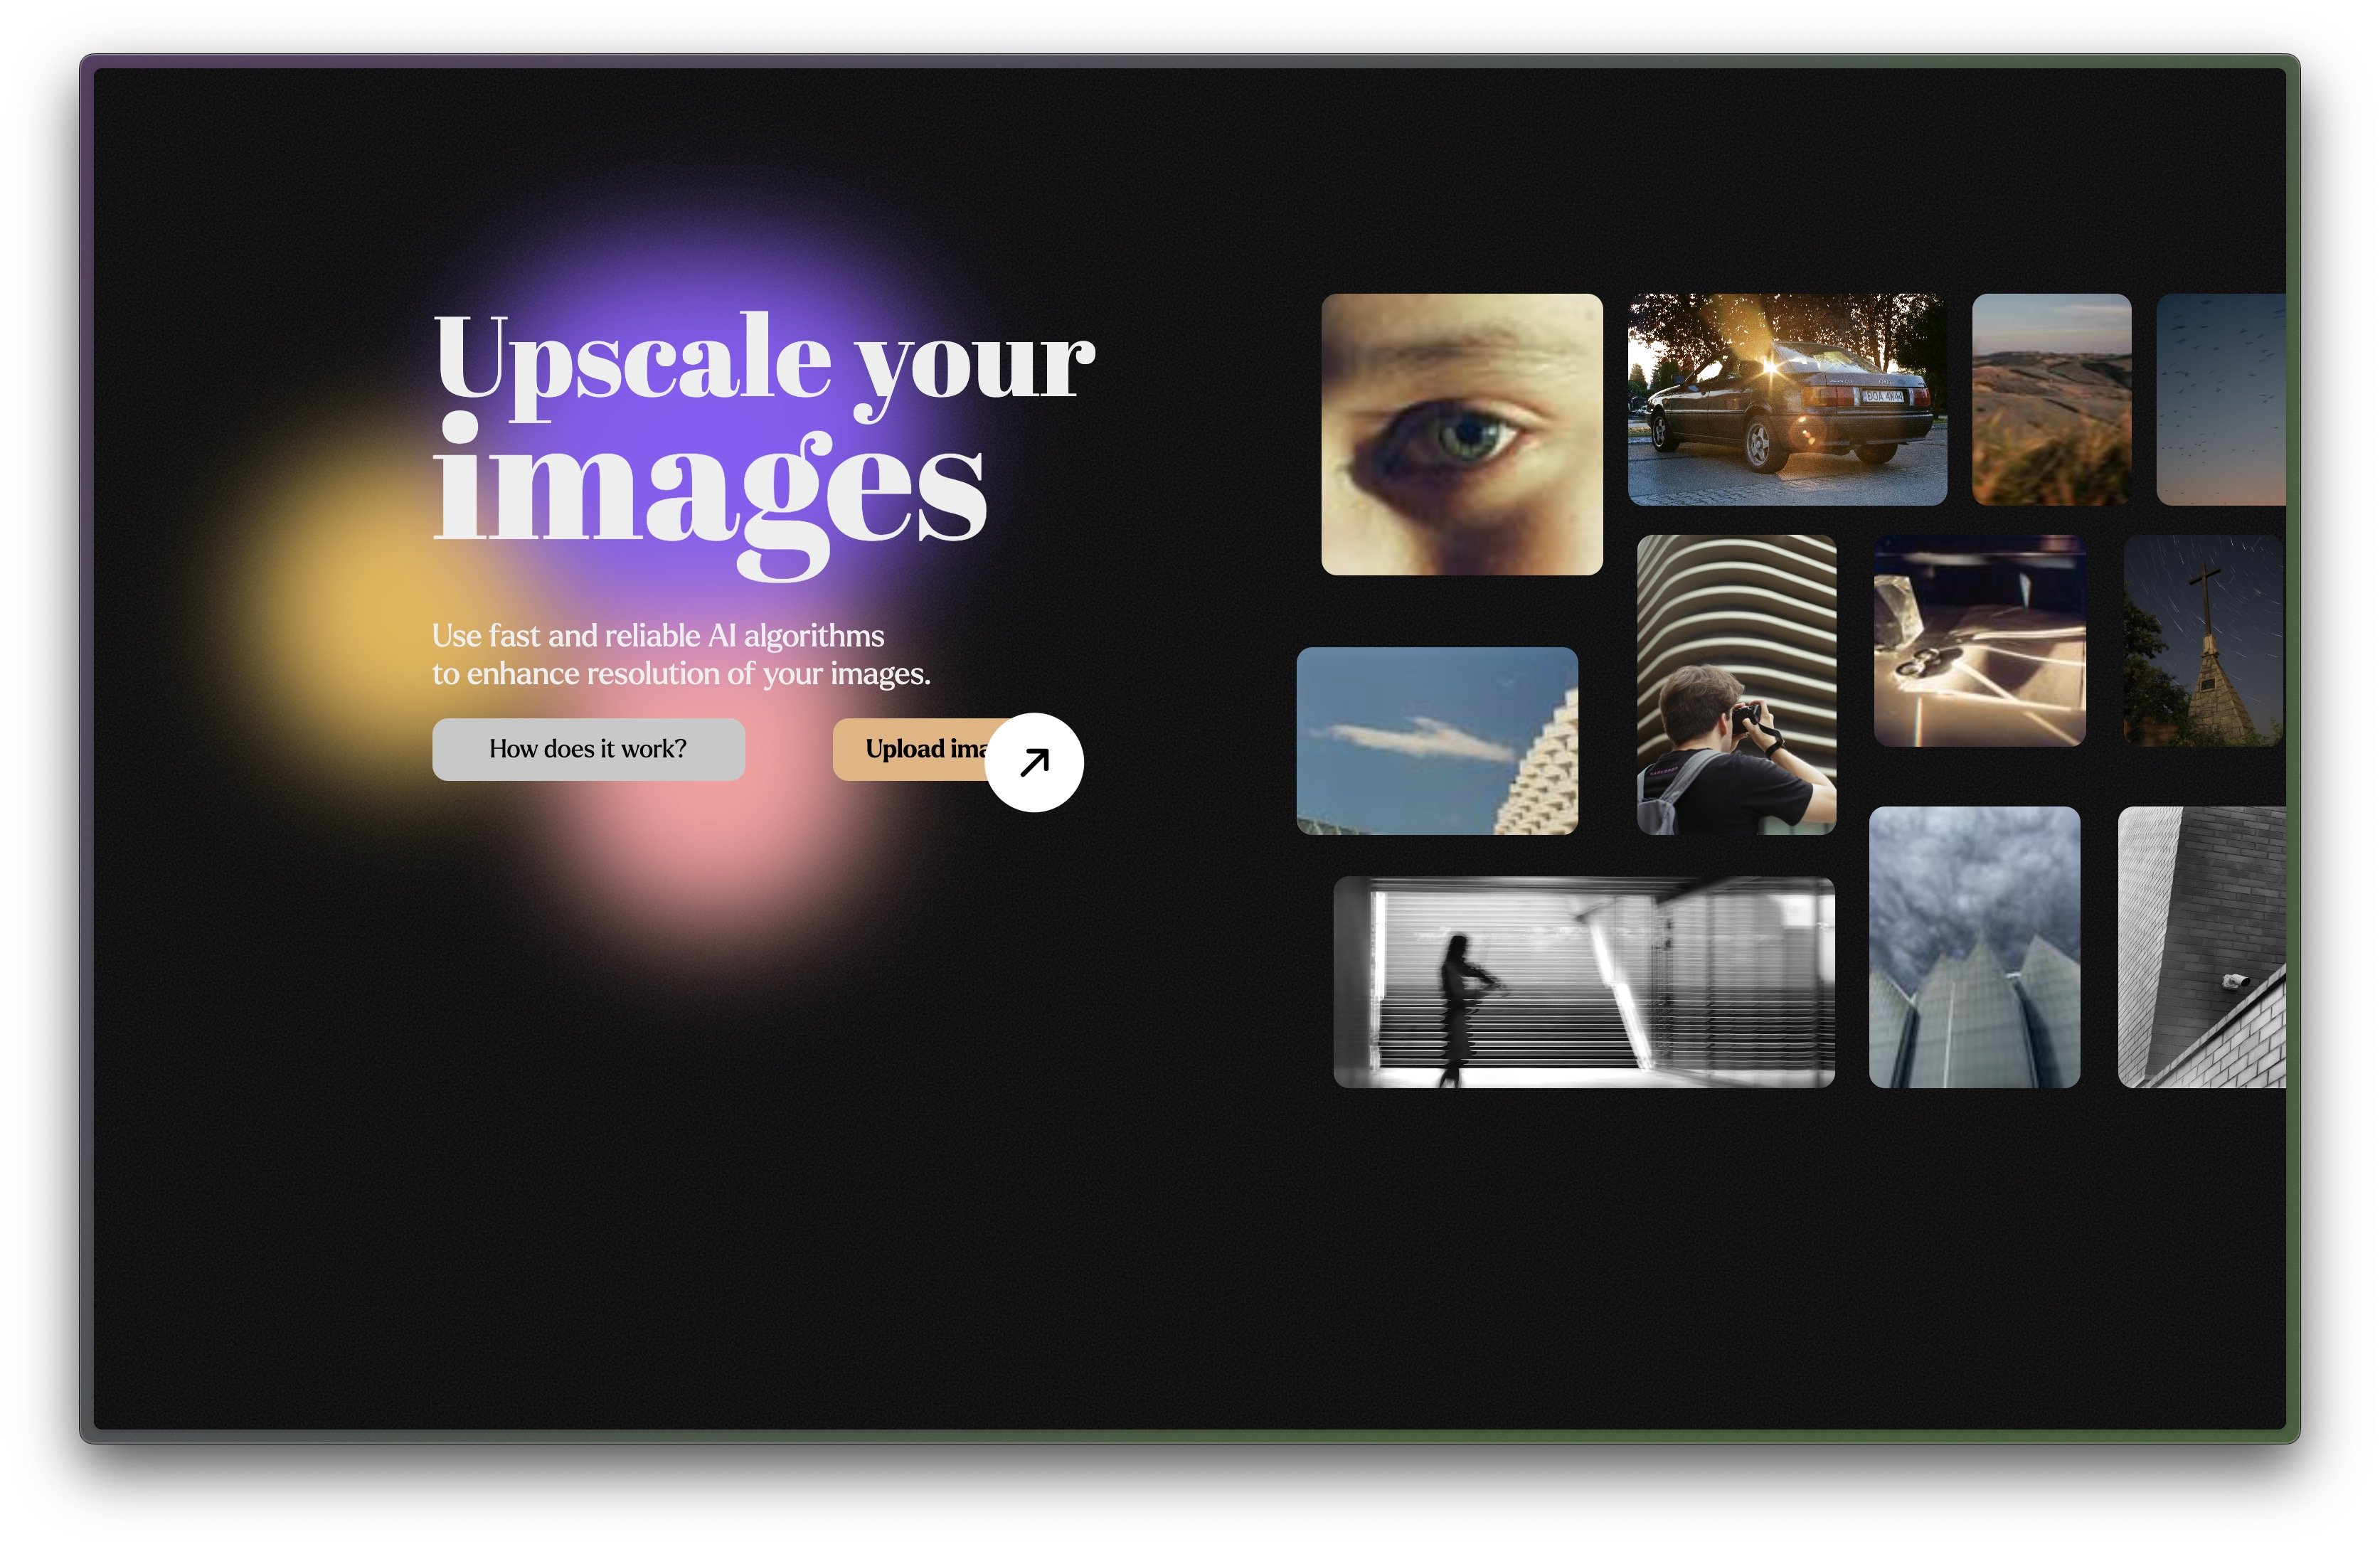
\includegraphics[width=\linewidth]{Rozdziały/06.Aplikacja/Obrazy/kursor-link.jpg}  
        \caption{Widok strony głównej aplikacji}
        \label{fig:image80}
        \hspace{2cm}
        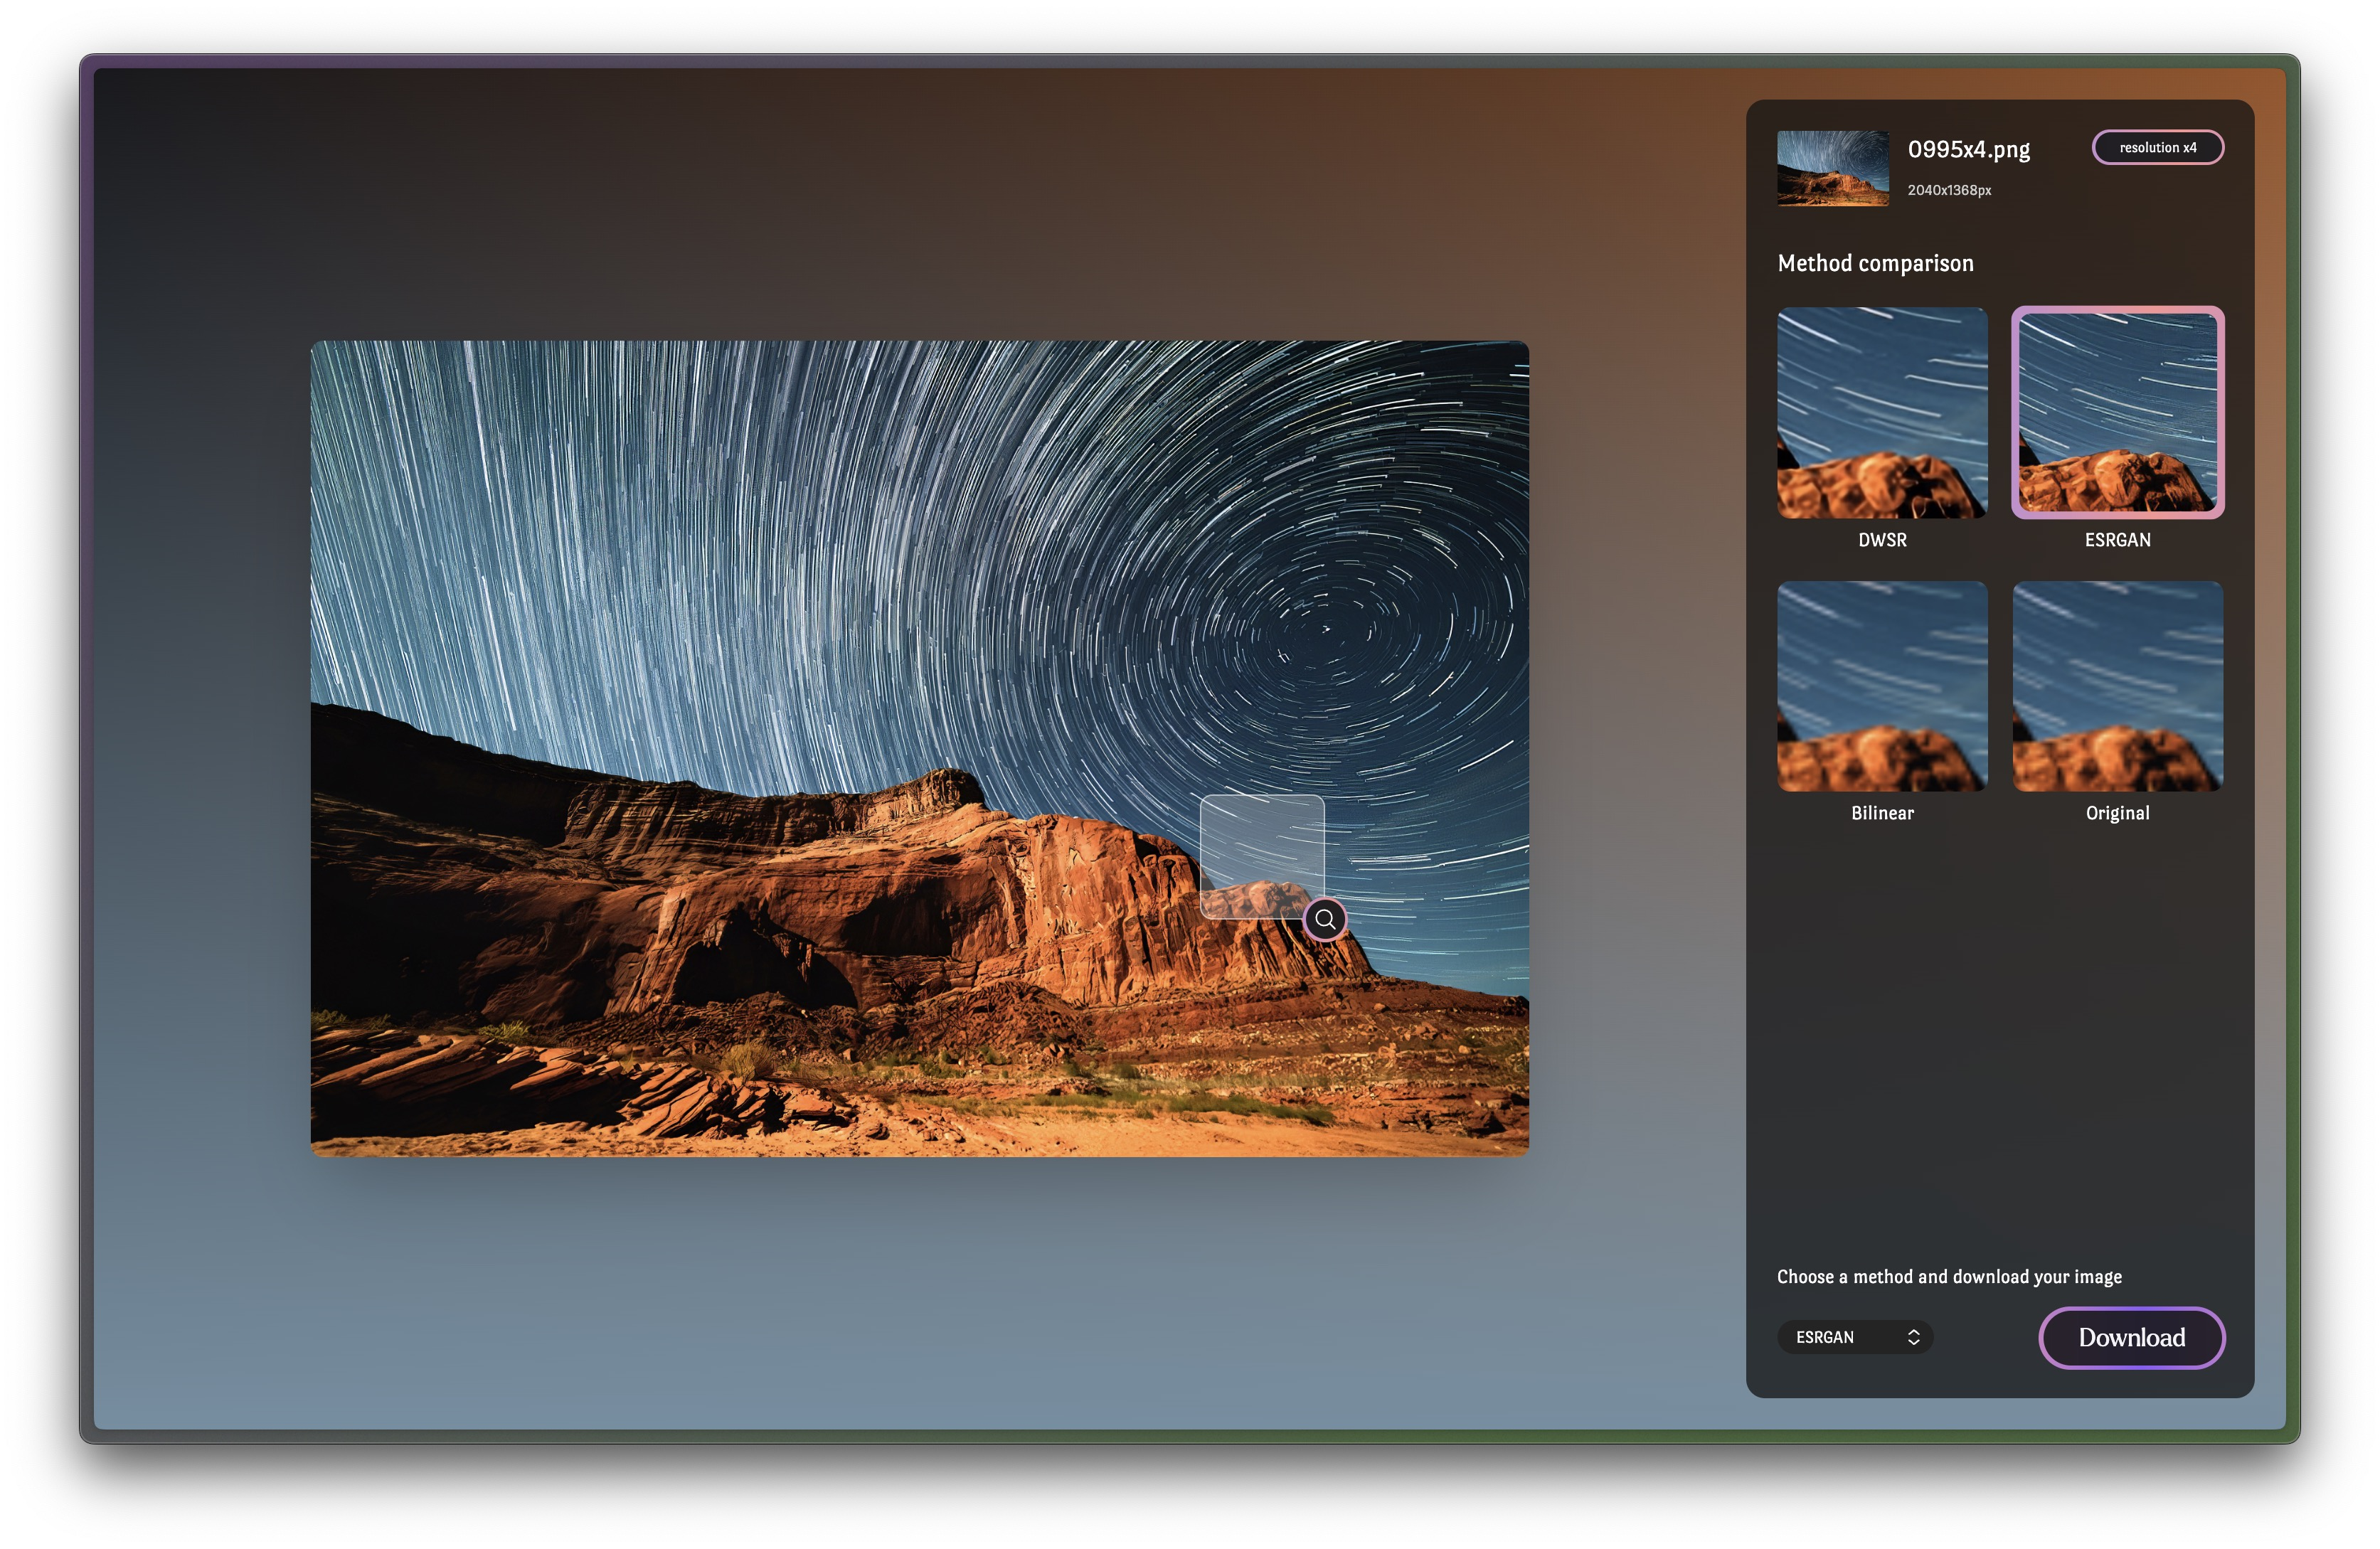
\includegraphics[width=\linewidth]{Rozdziały/06.Aplikacja/Obrazy/display5.jpg}  
        \caption{Widok prezentacji wyników (obraz z \cite{guo2017deep})}
        \label{fig:image81}
    \end{minipage}
\end{figure}
\newpage

\section{Projektowanie aplikacji}

Pierwszym etapem tworzenia aplikacji było stworzenie diagramu przepływu użytkownika (user flow diagram) [Rys \ref{fig:image82}], który ilustruje kolejność interakcji użytkownika z aplikacją. Potencjalni użytkownicy mają już pewne oczekiwania i potrzeby, spodziewają się gdzie na ekranie znajdą się konkretne elementy. Dlatego ważne jest, żeby zrozumieć jak użytkownik będzie korzystał z aplikacji, jakie akcje będzie wykonywał i w jaki sposób będzie się poruszał po stronie.

\begin{figure}[ht]
    \centering
    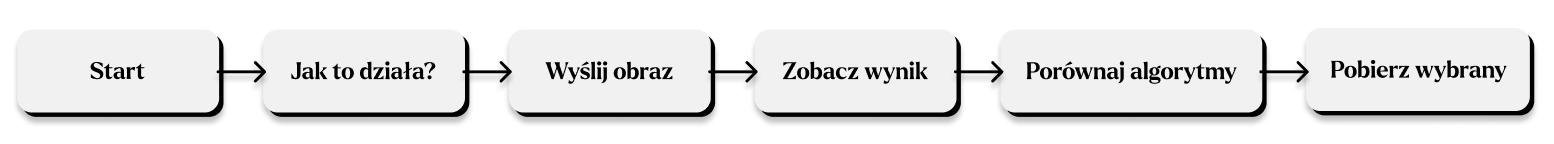
\includegraphics[width=\linewidth]{Rozdziały/06.Aplikacja/Obrazy/user-flow.png}  
    \caption{Diagram przepływu użytkownika}
    \label{fig:image82}
\end{figure}

Diagram ten przedstawia wszystkie interakcje, które użytkownik może wykonać w aplikacji. Te interakcje nie muszą być wykorzystane, ale są dostępne dla użytkownika.

Kolejnym krokiem był projekt interfejsu użytkownika. Zdecydowałem, że narzędzie będzie składać się z dwóch ekranów: ekranu głównego \ref{fig:image80}, oraz widoku prezentacji obrazu wynikowego \ref{fig:image81}.

Projekt wyglądu aplikacji rozpocząłem od rozrysowania wireframe'ów [Rys \ref{fig:image83}] z użyciem narzędzia \textbf{Figma}, służącym do projektów graficznych między innymi aplikacji. Wireframe'y to proste szkice, które pozwalają na zobrazowanie układu elementów na stronie. Elementy te odpowiadają za funkcjonalność, a nie wygląd aplikacji i są ściśle powiązane z diagramem przepływu użytkownika.

\begin{figure}[ht]
    \centering
    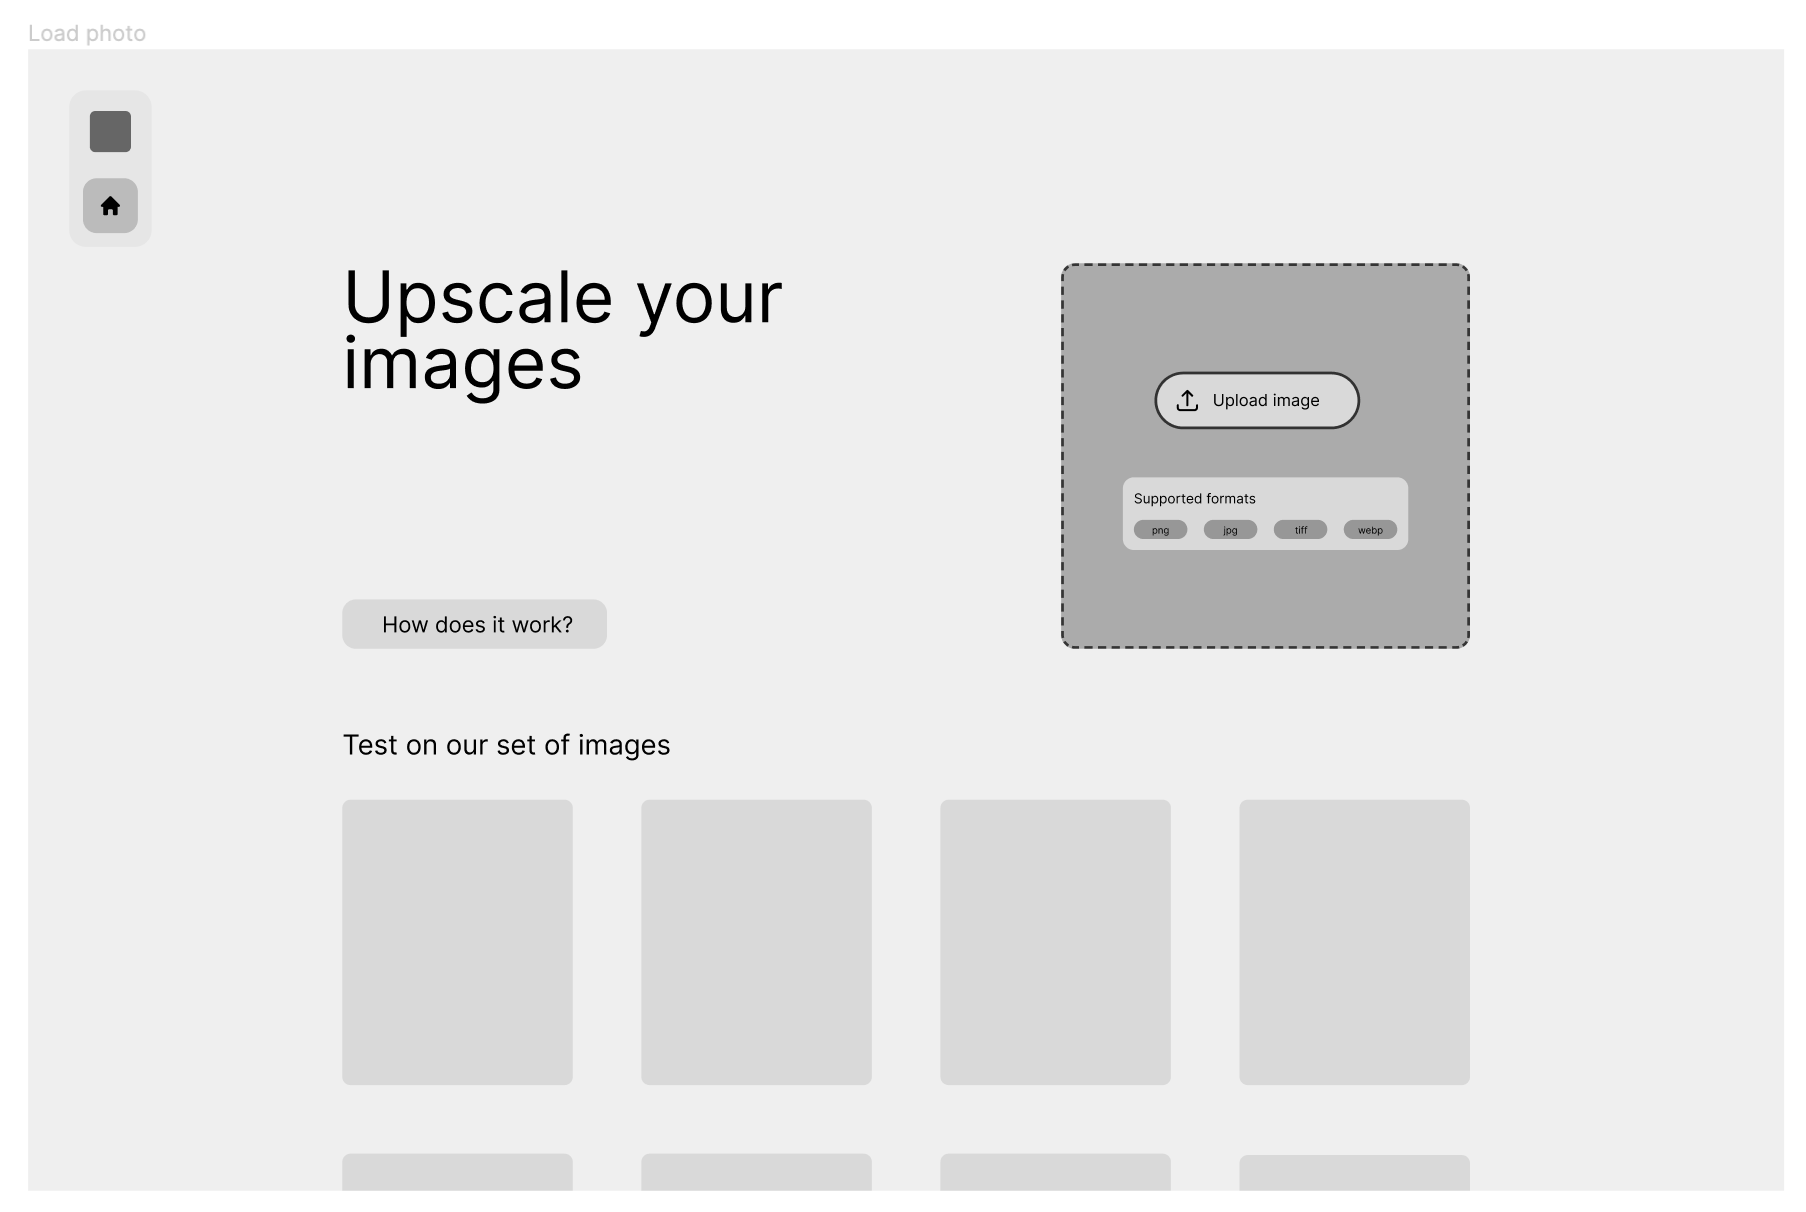
\includegraphics[width=0.8\linewidth]{Rozdziały/06.Aplikacja/Obrazy/UX upload.png}  
    \caption{Pierwsza wersja UX aplikacji (ekran główny)}
    \label{fig:image83}
\end{figure}

\begin{figure}[ht]
    \centering
    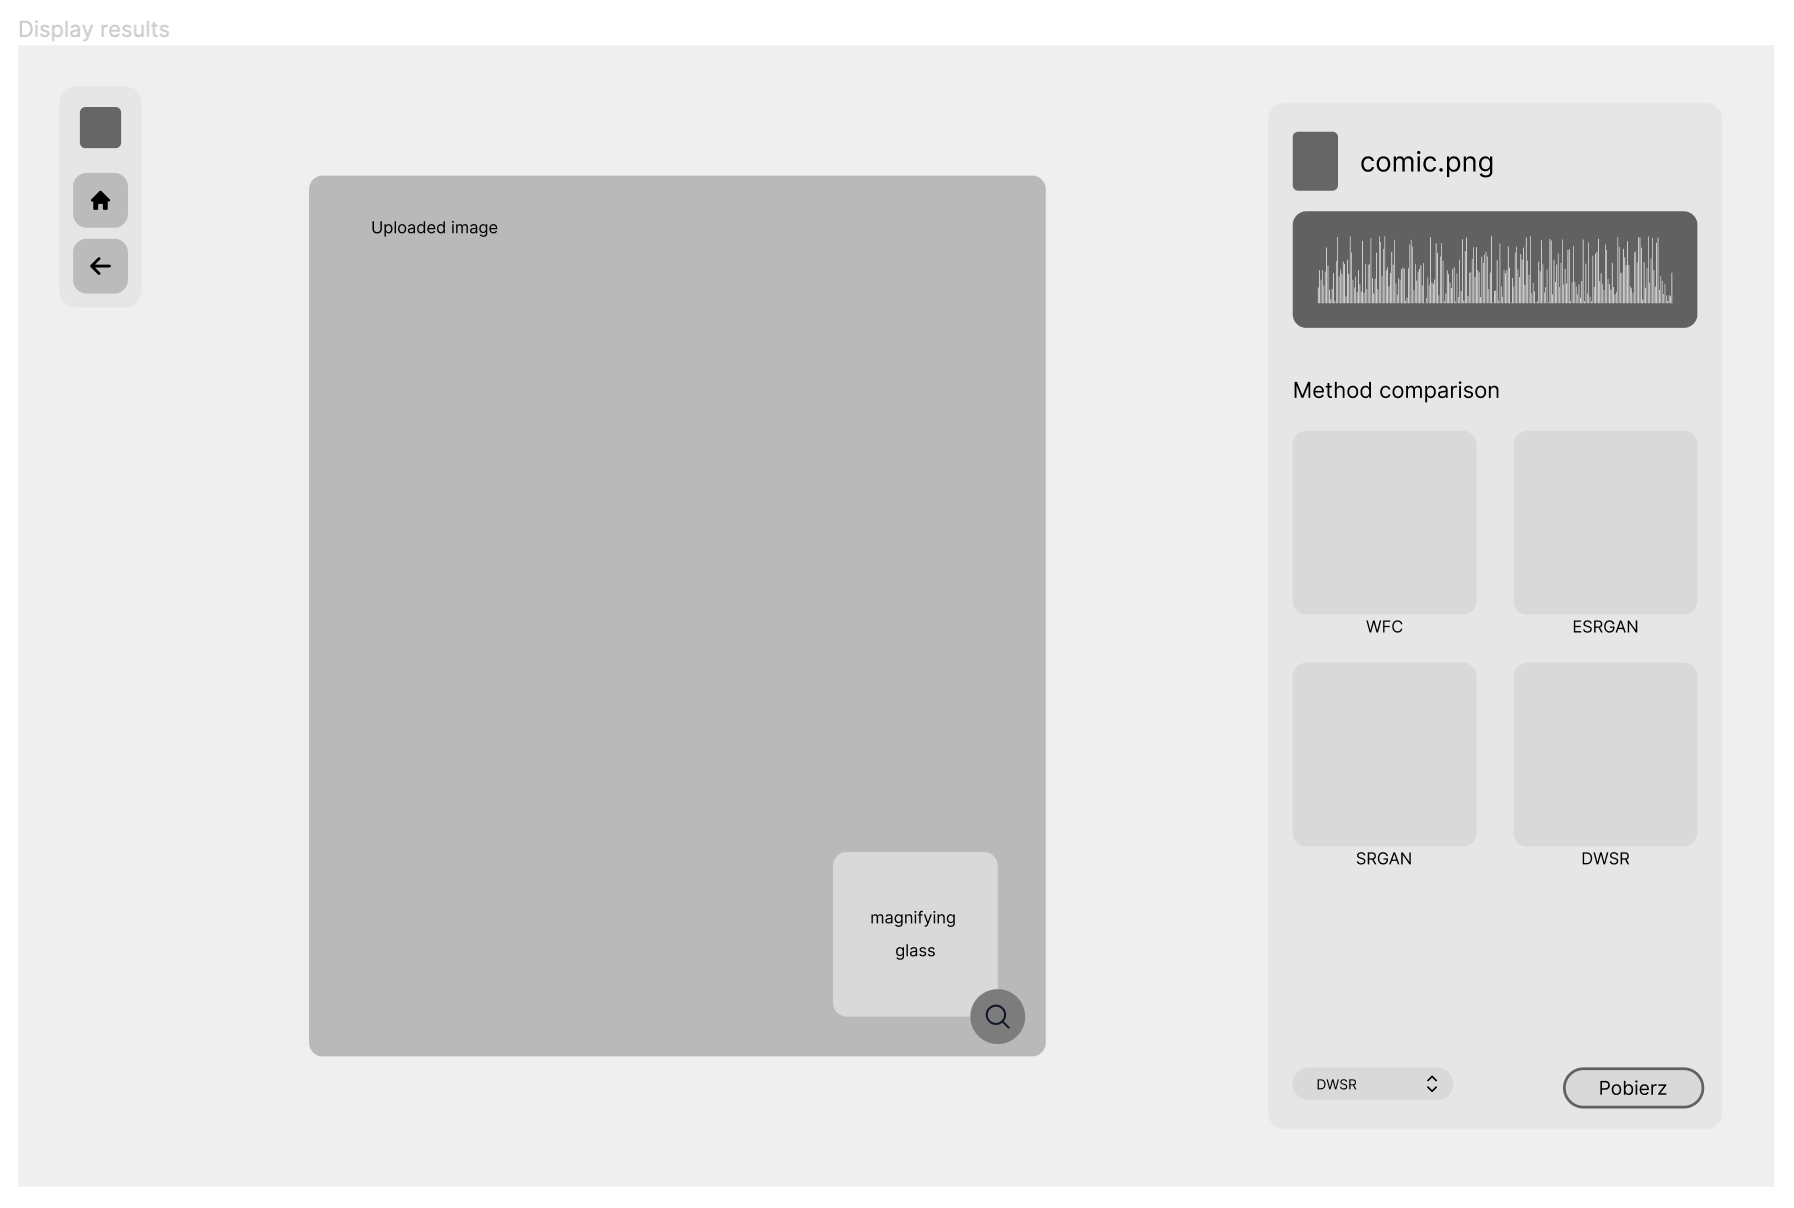
\includegraphics[width=0.8\linewidth]{Rozdziały/06.Aplikacja/Obrazy/UX display.png}  
    \caption{Pierwsza wersja UX aplikacji (ekran prezentacji wyników)}
    \label{fig:image84}
\end{figure}

Pierwotny rozkład elementów na stronie różni się od tego jak to wygląda teraz. Wraz z rozwojem aplikacji zmieniałem układ elementów, usprawniałem interakcję z użytkownikiem i poprawiałem rozkład elementów na ekranach aplikacji.

Kolejnym etapem pracy był projekt graficzny aplikacji. Zdecydowałem, że aplikacja będzie w ciemnym motywie, gdyż taki styl pomaga nam skupić się na tym co jest na ekranie, zwłaszcza w kontekście edycji zdjęć. Zależało mi na tym, żeby aplikacja nie była jednowymiarowa i żeby wyglądała nowocześnie. Początkowo eksperymentowałem z grafikami wektorowymi w tle [Rys \ref{fig:image85}], lecz ten wygląd nie przekonywał mnie. Eksperymentując z wyglądem pomyślałem, że w nawiązaniu do szumu na zdjęciach analogowych, tło aplikacji może mieć szum, zaś jako że mamy do czynienia z nowoczesnym narzędziem to kursor i elementy UI będą przejrzyste i czyste. W ten sposób aplikacja zyskuje na głębi i tak wygląda aktualna wersja, którą postanowiłem zaimplementować [Rys \ref{fig:image80}].

\begin{figure}[H]
    \centering
    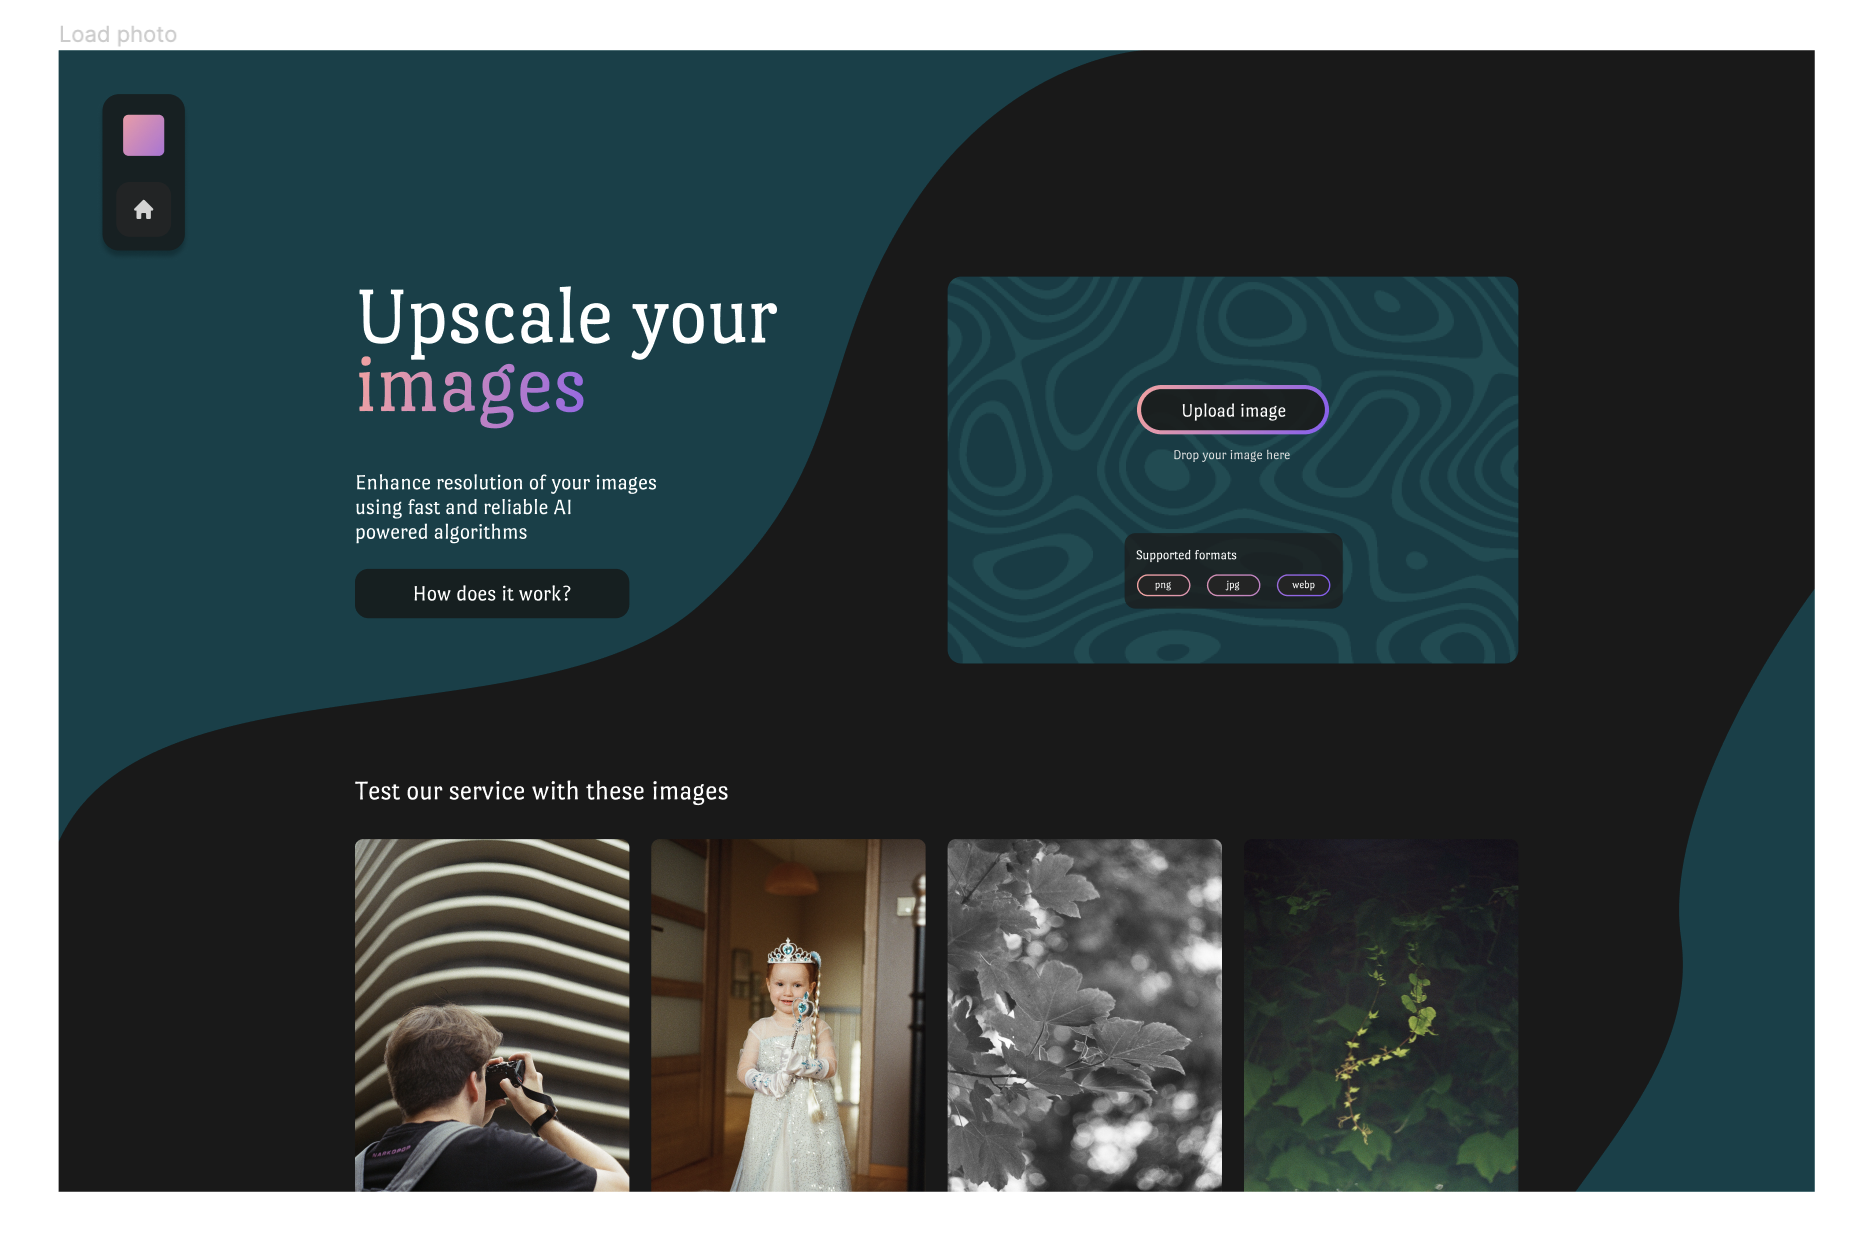
\includegraphics[width=0.8\linewidth]{Rozdziały/06.Aplikacja/Obrazy/UI 1.png}  
    \caption{Pierwsza wersja UI strony głównej}
    \label{fig:image85}
\end{figure}

Podobnie wyglądał proces projektowania ekranu prezentacji wyników [Rys \ref{fig:image86}]. Zdecydowałem, żeby na ekranie prezentacji wyników były tylko istotne elementy interfejsu, żeby użytkownik nie pogubił się w nadmiarze informacji. Zależało mi na tym, żeby użytkownik mógł łatwo porównać wyniki różnych algorytmów, dlatego zdecydowałem się na układ kafelków, które można wybrać i porównać z sobą. Dodatkowo w tych kafelkach uznałem, że świetnie sprawdzi się widok z bliska, który pozwoli na dokładne przyjrzenie się szczegółom obrazu, tak powstała lupka, która podąża za kursorem gdy wskaźnik znajduje się nad obrazem. 


\begin{figure}[H]
    \centering
    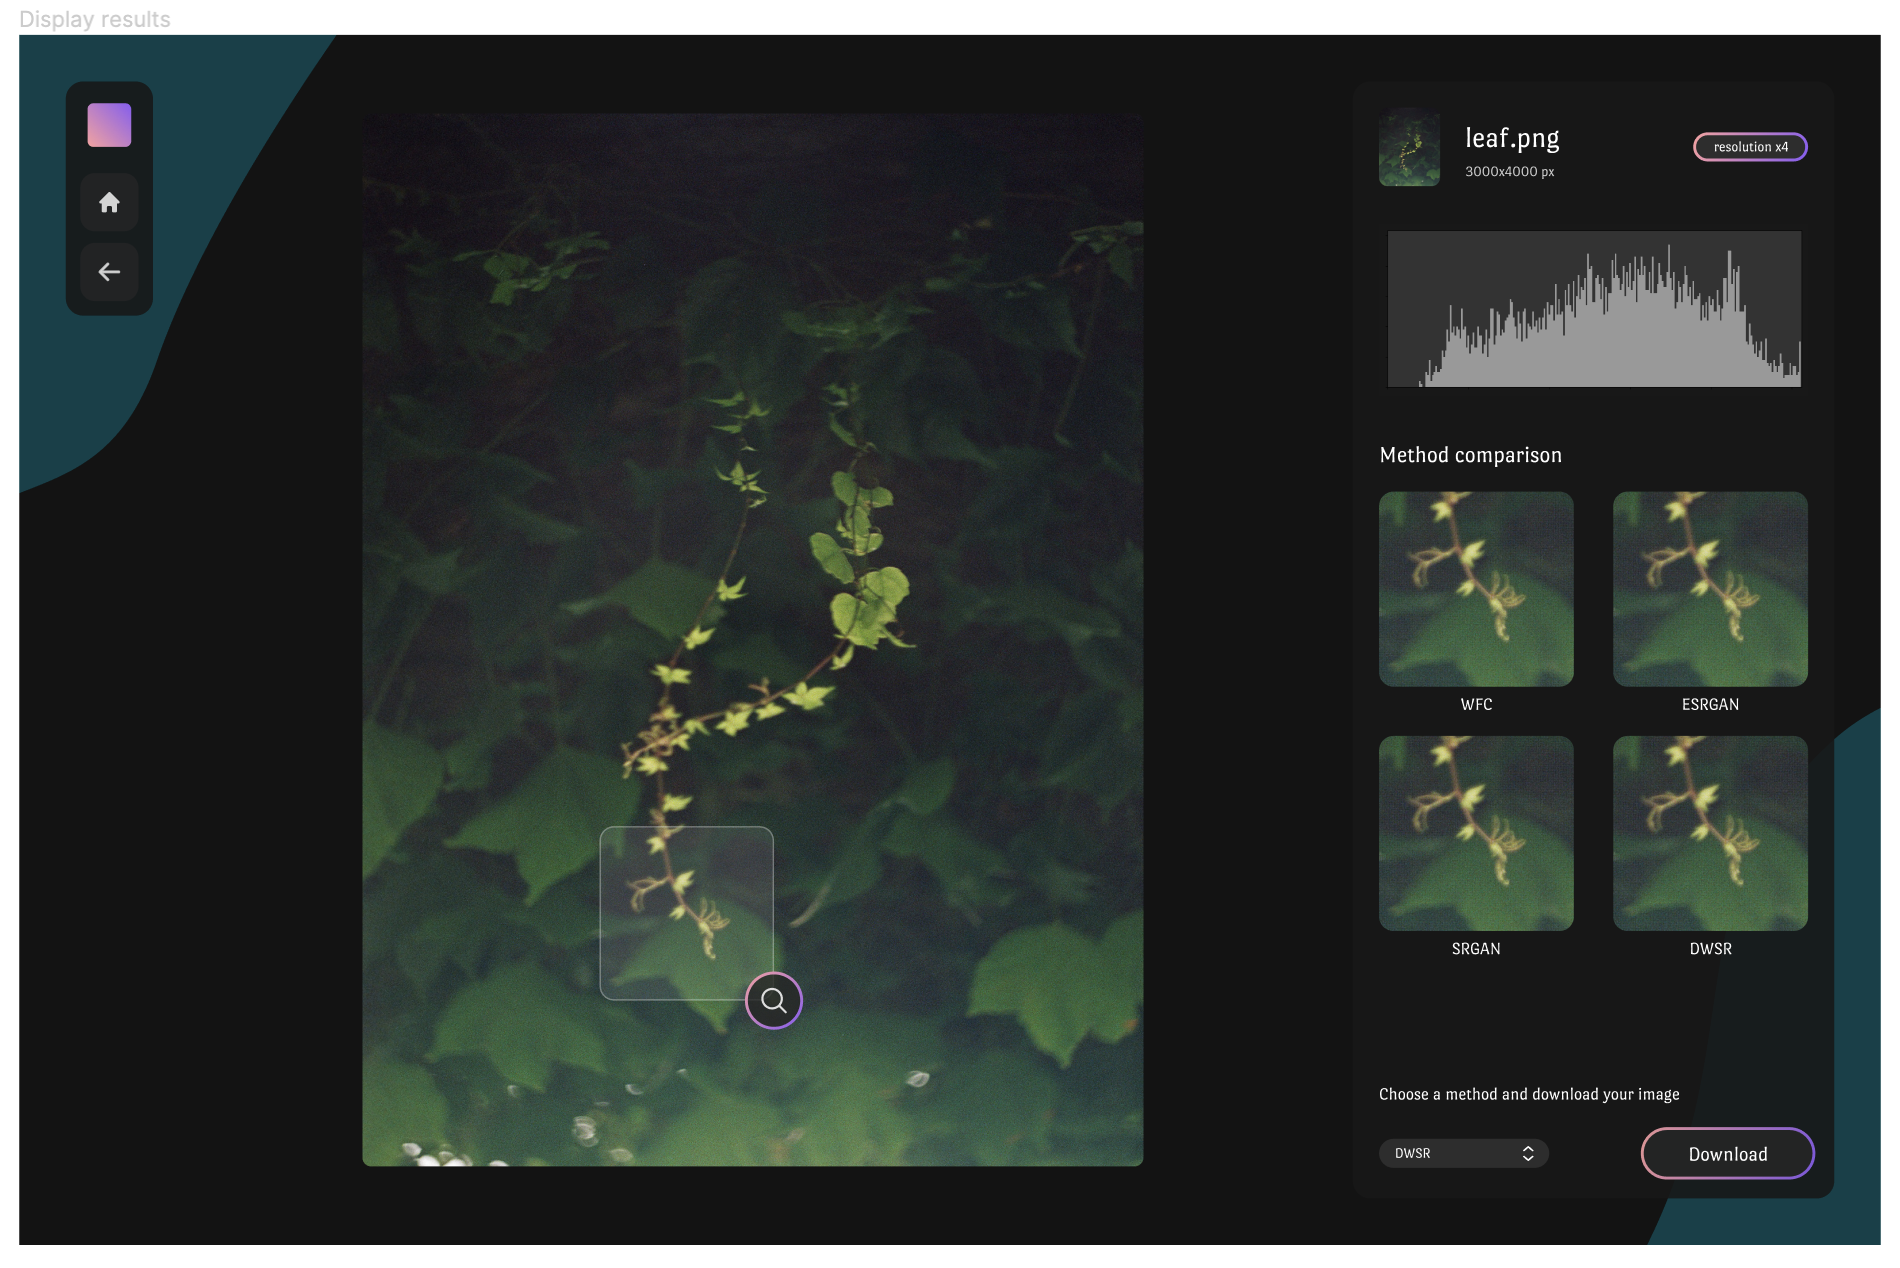
\includegraphics[width=0.8\linewidth]{Rozdziały/06.Aplikacja/Obrazy/UI 1 dsiplay .png}  
    \caption{Pierwsza wersja UI ekranu wyświetlania wyników}
    \label{fig:image86}
\end{figure}

W kolejnej wersji widoku prezentacji wyników postanowiłem zmienić wygląd tła. Zainspirowany aplikacjami typu \textbf{Apple Music} czy \textbf{Spotify} zdecydowałem się na zmianę tła na gradient z kolorów występujących na obrazie. W ten sposób aplikacja zyskuje na głębi i wygląda bardziej nowocześnie [Rys \ref{fig:image81}]. W tym miejscu projekt aplikacji uznałem za gotowy do implementacji, gdzieś trzeba się zatrzymać, żeby sprawdzić jak działają mechanizmy w praktyce. O planach rozbudowy aplikacji traktuję rozdział \ref{sec:plans}.



\section{Wybór narzędzi i technologii}

Kolejnym krokiem w tworzeniu aplikacji jest decyzja odnośnie używanych technologii i narzędzi. W tym rozdziale opiszę jakie technologie wybrałem do stworzenia aplikacji webowej. 

Aplikacja dzieli się na Frontend i Backend, gdyż zadanie Super-Rozdzielczości, podobnie jak inne zadania z dziedziny uczenia maszynowego, wymaga dużej mocy obliczeniowej. Z tego powodu implementowane algorytmy będą działać po stronie Backendu, a Frontend będzie odpowiedzialny za interfejs użytkownika, wyświetlenie wyników i komunikację z Backendem. 
Dodatkowo Backend pozwala na przechowywanie obrazów w bazie danych, co jest istotne gdy chcemy porównać wyniki różnych algorytmów ze sobą od strony administratora.


\section{Vue.js: Frontend}

Do implementacji Frontendu zdecydowałem się na użycie frameworku \textbf{Vue.js} \cite{vusjs}.


\textbf{Vue.js} to progresywny framework JavaScript służący do budowania interfejsów użytkownika. Został stworzony przez Evana You i jest utrzymywany przez niezależnych współtwórców z całego świata. Jego elastyczność pozwala na łatwą integrację z innymi bibliotekami lub istniejącymi projektami, a także jest świetny do tworzenia zaawansowanych aplikacji jednostronicowych (SPA - Single Page Applications). Swietnie nada się do tego projektu, gdyż jest to niewielka aplikacja, która będzie korzystać z wielu bibliotek i narzędzi. W kolejnych podrozdziałach opiszę dlaczego Vue.js jest dobrym wyborem do tego projektu.


\subsubsection*{Architektura i Komponenty}

Architektura Vue opiera się na systemie komponentów. Komponenty w Vue są blokami wielokrotnego użytku z własnym stanem, metodami i szablonami. Dzięki temu łatwo jest tworzyć interfejsy składające się z mniejszych, niezależnych części, co znacznie ułatwia zarządzanie, utrzymanie i czytelność kodu.

\subsubsection*{Reaktywność i Dwukierunkowe Wiązanie Danych}

Jedną z kluczowych cech Vue.js jest jego reaktywny system, który zapewnia automatyczną aktualizację interfejsu użytkownika w odpowiedzi na zmiany stanu aplikacji. Framework ten używa systemu dwukierunkowego wiązania danych (two-way data binding), co oznacza, że zmiany w modelu danych od razu są odzwierciedlane w widoku i na odwrót.

\subsubsection*{Deklaratywne Renderowanie}

Vue.js wykorzystuje deklaratywne renderowanie. Oznacza to, że developer określa, jakie dane powinny być wyświetlane, a framework zajmuje się ich aktualizacją w widoku. To sprawia, że kod jest bardziej zrozumiały i łatwiejszy w utrzymaniu.

\subsubsection*{Virtual DOM}

Vue korzysta z koncepcji Virtual DOM, co pozwala na efektywną aktualizację widoku bez konieczności odświeżania całej strony. Jest to znacznie szybsze niż tradycyjne manipulowanie DOM, ponieważ zmiany są najpierw aplikowane do Virtual DOM, a następnie, w optymalny sposób, przekazywane do rzeczywistego DOM.

\subsubsection*{Ekosystem i Społeczność}

Vue ma rozbudowany ekosystem, w skład którego wchodzą takie narzędzia jak Vue Router (do zarządzania nawigacją w aplikacji) i Vuex (do zarządzania stanem aplikacji). Dodatkowo, wsparcie społeczności i dostępność zasobów edukacyjnych, takich jak dokumentacja, poradniki i fora dyskusyjne, sprawiają, że nauka i praca z Vue.js jest dostępna i przyjemna.


\newpage
\section{Django: Backend}

Do implementacji Backendu zdecydowałem się na użycie frameworku \textbf{Django} \cite{django}.

\textbf{Django} to wysokopoziomowy framework webowy napisany w Pythonie, który umożliwia szybkie tworzenie bezpiecznych i łatwych w utrzymaniu stron internetowych. Został zaprojektowany z myślą o uproszczeniu zadań związanych z tworzeniem aplikacji internetowych, dzięki czemu deweloperzy mogą skupić się po prostu na pisaniu aplikacji. W kolejnych podrozdziałach opiszę dlaczego Django jest dobrym wyborem do tego projektu.


\subsubsection*{Python}

Django jest napisane w języku Python, który jest jednym z najpopularniejszych i najbardziej lubianych języków programowania. W języku tym zostały zaimplementowane algorytmy DWSR i ESRGAN, więc wykorzystanie Django pozwoli na łatwą integrację tych algorytmów z aplikacją.

\subsubsection*{Architektura Wzorca Projektowego MTV}

Django wykorzystuje wzorzec projektowy "Model-Template-View" (MTV), który jest podobny do popularnego wzorca MVC. W tym podejściu:
\begin{itemize}
    \item \textbf{Model} odpowiada za strukturę danych oraz ich walidację.
    \item \textbf{Template} odpowiada za prezentację danych.
    \item \textbf{View} odpowiada za logikę aplikacji, odbierając żądania od użytkownika i zwracając odpowiednie odpowiedzi.
\end{itemize}

W tego typu projektach warto stosować wzorce projektowe, ponieważ ułatwiają one zarządzanie kodem i zwiększają jego czytelność. Ponadto, stosowanie wzorców projektowych jest dobrym zwyczajem, który pozwala na łatwiejsze utrzymanie aplikacji w przyszłości.

\subsubsection*{ORM (Object-Relational Mapping)}

Django zawiera wbudowany ORM, który pozwala na interakcję z bazami danych za pomocą kodu Python, zamiast pisać surowe zapytania SQL. ORM przekształca tabele bazy danych w klasy Pythona, co ułatwia manipulowanie danymi i sprawia, że kod jest bardziej czytelny, prostszy w zarządzaniu i łatwiejszy w utrzymaniu.

\subsubsection*{Wbudowane Funkcje}

Django oferuje wiele wbudowanych funkcji, takich jak system uwierzytelniania użytkowników, mapowanie URL na widoki, mechanizm szablonów, system administrowania itd. Dzięki temu można szybko rozpocząć pracę nad projektem, mając już na starcie zestaw potrzebnych narzędzi.


\subsubsection*{Skalowalność}

Django jest skalowalny i może obsługiwać zarówno małe, jak i duże projekty. Ponadto, framework ten wspiera koncept wersjonowania API, co jest kluczowe przy rozwijaniu i utrzymywaniu dużych aplikacji.

\subsubsection*{Wsparcie Społeczności i Dokumentacji}

Podobnie jak w przypadku Vue.js, Django ma silną i aktywną społeczność. Dzięki temu deweloperzy mają dostęp do bogatej dokumentacji, licznych zasobów edukacyjnych i gotowych rozwiązań, co ułatwia naukę i rozwiązywanie problemów.


\section{Implementacja aplikacji}

Po wyborze stosu technologicznego kolejnym krokiem jest skupienie się na implementacji rozwiązań. W tym rozdziale opiszę jakie decyzje podjąłem przy pisaniu kodu aplikacji, jak wygląda jej struktura i jakie problemy napotkałem podczas implementacji.

\subsection*{Struktura aplikacji}

Aplikacja składa się z dwóch części - Frontendu i Backendu. Przy tworzeniu takiego projektu warto zadbać o to, żeby każda część była od siebie niezależna i żeby komunikacja między nimi była jak najmniej skomplikowana.

W tym miejscu wracamy do diagramu przepływu użytkownika [Rys \ref{fig:image82}], jak na nim widać użytkownik nie może wykonać zbyt wiele akcji, struktura aplikacji jest liniowa. Na podstawie diagramu przepływu użytkownika można stworzyć schemat blokowy aplikacji [Rys \ref{fig:image87}], który pozwoli zrozumieć zachowanie programu.

\begin{figure}[H]
    \centering
    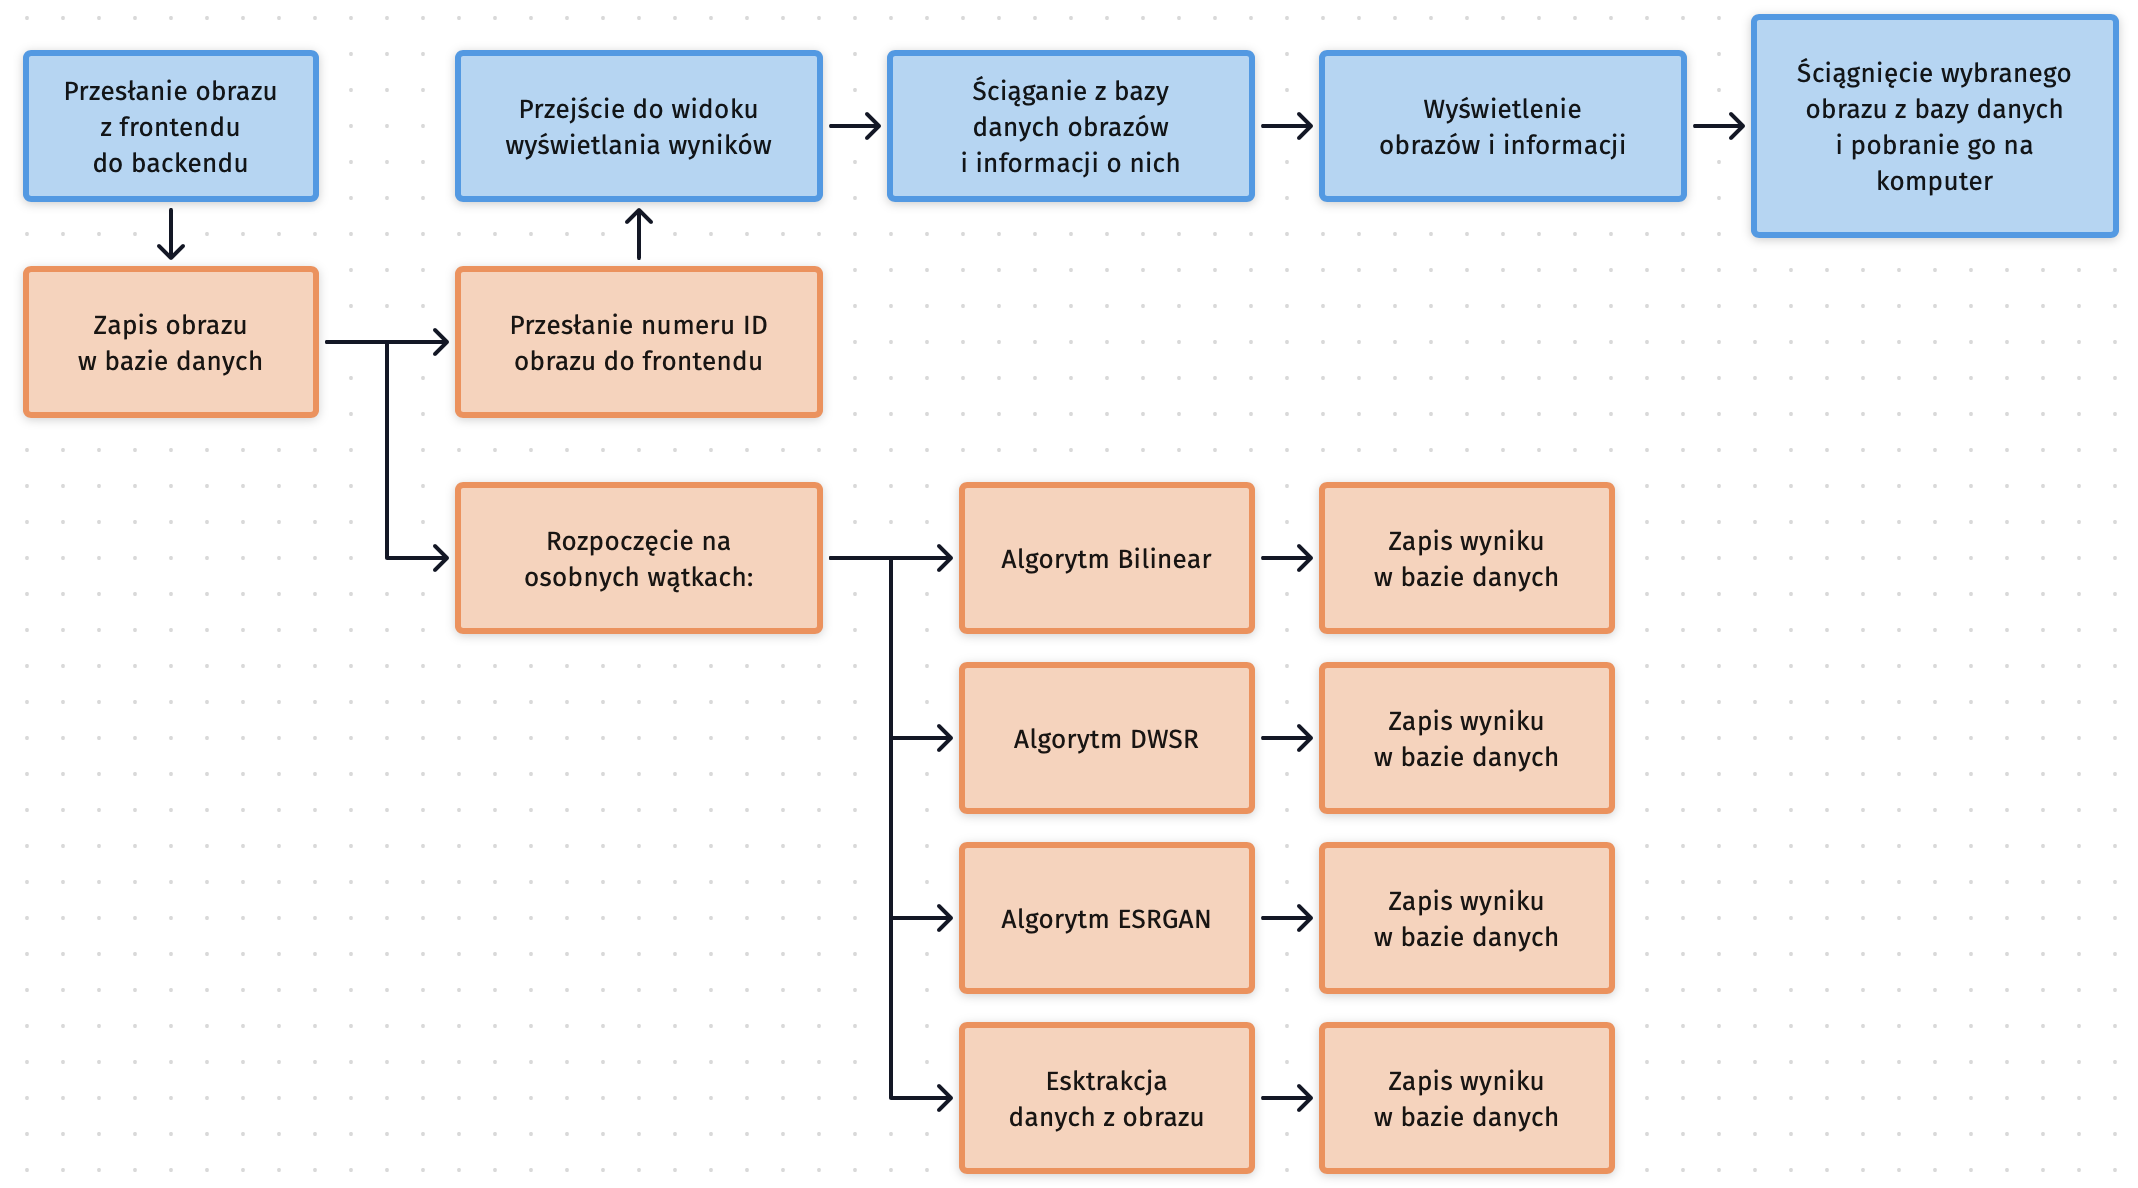
\includegraphics[width=\linewidth]{Rozdziały/06.Aplikacja/Obrazy/mechanizm_aplikacji.png}  
    \caption{Schemat blokowy aplikacji (kolor niebieski - Frontend, pomarańczowy - Backend)}
    \label{fig:image87}
\end{figure}

W pierwszej kolejności użytkownik wysyła obraz do serwera Backend, który zapisuje go w bazie danych. Następnie serwer zleca wykonanie algorytmów na osobnych wątkach, o czym opowiem w dalszej części rozdziału [\ref{sec:implementation-s-r}]. Gdy algorytmy rozpoczną pracę, serwer zwraca do Frontendu informację o tym że operacja zapisu się powiodła i podaje numer ID obrazu. 

Frontend zmienia widok na ten z wynikami i wysyła zapytanie do Backendu o obraz oryginalny i przetworzone. Następnie jeśli serwer zwróci obrazy, Frontend je wyświetla. W przeciwnym wypadku próbuje je pozyskać ponownie aż do skutku. Dzieje się tak, dlatego że zadanie super-rozdzielczości jest czasochłonne i czasem może zająć kilka sekund a w innych wypadkach nawet kilka minut, wszystko w zależności od rozdzielczości obrazów. W tym czasie użytkownik może porównywać uzyskane wyniki i wybrać najlepszy. 

Gdy użytkownik wybierze obraz, może go pobrać na swój komputer. Wtedy Frontend wysyła zapytanie do serwera o obraz w pełnej rozdzielczości, a serwer zwraca obraz, który przeglądarka automatycznie pobiera.

\subsubsection*{Architektura bazy danych}

Baza danych w aplikacji jest bardzo prosta, przy przesłaniu każdego zdjęcia w bazie tworzone jest pole Image, które przechowuje informacje o obrazie oraz jego przetworzonych wersjach. W tabeli \ref{tab:image_model} przedstawiam jedyną tabelę w bazie danych, która przechowuje informacje o obrazach.

\begin{table}[ht]
    \centering
    \renewcommand{\arraystretch}{1.5} % Increase row height by 1.25 times
    \begin{tabular}{|l|l|p{8cm}|}
    \hline
    \multicolumn{3}{|c|}{\textbf{Image}}                                                        \\ \hline
    \textbf{Pole}       & \textbf{Typ}          & \textbf{Opis}                                 \\ \hline
    image               & ImageField            & Przesłany obraz.                              \\ \hline
    bilinear\_image     & ImageField            & Obraz powiększony algorytmem Bilinear.        \\ \hline
    dwsr\_image         & ImageField            & Obraz powiększony algorytmem DWSR.            \\ \hline
    esrgan\_image       & ImageField            & Obraz powiększony algorytmem ESRGAN.          \\ \hline
    original\_height    & PositiveIntegerField  & Wysokość oryginalnego obrazu.                 \\ \hline
    original\_width     & PositiveIntegerField  & Szerokość oryginalnego obrazu.                \\ \hline
    dominant\_colors    & TextField             & Pole tekstowe z listą dominujących kolorów.   \\ \hline
    \end{tabular}
    \caption{Struktura bazy danych - Image.}
    \label{tab:image_model}
\end{table}

Jak widać w bazie danych przechowywane są obrazy w formacie \textit{ImageField}, który jest dostarczany przez bibliotekę Django. Jest to pole, które przechowuje ścieżkę do pliku na dysku serwera. Zapisujemy również informacje o oryginalnych wymiarach obrazu, które są wyświetlane użytkownikowi przez Frontend. 

Dodatkowo w bazie danych przechowujemy listę dominujących kolorów, które są wykrywane przez algorytm K-średnie \textit{K-means} \cite{sklearn} , o którym opowiem w kolejnym rozdziale [\ref{sec:implementation-s-r}]. Jest to lista kolorów w formacie HEX, które wykorzystuje Frontend do wyświetlenia kolorowych gradientów tła.



\section{Integracja algorytmów super-rozdzielczości} \label{sec:implementation-s-r}

Gdy obraz jest już zapisany w bazie danych, serwer Backend zleca wykonanie algorytmów super-rozdzielczości na osobnych wątkach [\ref{lst:save_image}]. W tym rozdziale opiszę w jaki sposób zostały zaimplementowane algorytmy w aplikacji.

W części Backendu aplikacji korzystam z bibliotek \textbf{OpenCV2} \cite{opencv}, \textbf{numpy} \cite{numpy}, \textbf{PyWavelets} \cite{pywavelets} oraz \textbf{PyTorch} \cite{pytorch}.

\newpage
\begin{lstlisting}[language=Python, caption=Obsługa zapisu i przetwarzania obrazów., label={lst:save_image}]
def upload_image(request):
try:
    form = Image(image=request.FILES['image'])
    form.save()

    input_image_path = form.image.path
    
    thread1 = threading.Thread(target = run_bilinear, 
                               args = (input_image_path, 4, form))
    thread2 = threading.Thread(target = run_dwsr, 
                               args = (input_image_path, 4, form))
    thread3 = threading.Thread(target = run_esrgan, 
                               args = (input_image_path, form))
    thread4 = threading.Thread(target = extract_image_info, 
                               args = (input_image_path, form))
    thread1.start()
    thread2.start()
    thread3.start()
    thread4.start()

    image = Image.objects.latest('id')  # Gets the latest entry

    return JsonResponse({'message': 'Image uploaded, processing started', 
                            'image_id': image.id})
except Exception as e:
    return JsonResponse({'error': str(e)}, status=400)
\end{lstlisting}

Stworzone zostały cztery funkcje - \textit{run\_bilinear}, \textit{run\_dwsr}, \textit{run\_esrgan} oraz\\ \textit{extract\_image\_info}. Pierwsze trzy z nich odpowiadają za uruchomienie algorytmów super-rozdzielczości, a ostatnia za wydobycie informacji o obrazie.




\subsection*{Algorytm Interpolacji Dwuliniowej}

Pierwszy z algorytmów, który został zaimplementowany to algorytm Interpolacji Dwuliniowej omawiany w rozdziale Podstawy Teoretyczne w sekcji \ref{sec:przeglad_metod_powiekszania_obrazow}.
Jest to najmniej skomplikowany algorytm, więc implementacja jego nie była trudna [\ref{lst:bilinear}].

\begin{lstlisting}[language=Python, caption=Implementacja algorytmu Bilinear., label={lst:bilinear}]
def run_bilinear(input_image_path, scale, image_instance):
    img = cv2.imread(input_image_path, cv2.IMREAD_COLOR)
    
    height, width = img.shape[:2]
    new_width, new_height = width * scale, height * scale

    # Resize the image using bilinear interpolation
    output = cv2.resize(img, (new_width, new_height), interpolation=cv2.INTER_LINEAR)

    save_output_image(output, input_image_path, image_instance)
\end{lstlisting}

Wczytujemy obraz do powiększenia, następnie pobieramy jego wymiary i mnożymy je przez skalę otrzymując nową wielkość obrazu. W kolejnym kroku wykorzystujemy funkcję \textit{cv2.resize} z biblioteki OpenCV2, która pozwala na zmianę rozmiaru obrazu. W tym miejscu wykorzystujemy parametr \textit{interpolation=cv2.INTER\_LINEAR}, który odpowiada za wybór algorytmu interpolacji. Na koniec zapisujemy obraz w bazie danych.


\subsection*{Algorytm DWSR}

Kolejnym algorytmem jest algorytm DWSR, który został opisany w rozdziale \ref{{chap:DWSR}}.
Implementacja tego algorytmu jest bardziej skomplikowana, ponieważ wymaga on zainstalowania modelu, który jest wykorzystywany do przetwarzania obrazów, oraz wymagała przepisania skryptów napisanych w Matlabie na język Python [\ref{lst:dwsr}].


\begin{lstlisting}[language=Python, caption=Implementacja algorytmu DWSR., label={lst:dwsr}]    
def run_dwsr(input_image_path, scale, image_instance):
    enlarged_lr_dir, sr_lum_dir, output_dir = create_output_dir()

    fileName = os.path.basename(input_image_path)

    # 1. Generate enlarged LR images
    generate_enlarged_lr(input_image_path, enlarged_lr_dir, scale) 

    # 2. Process image with DWSR
    process_image(enlarged_lr_dir + '/' + fileName, sr_lum_dir, scale)

    # 3. Generate color SR
    final_img_path = generate_color_sr(input_image_path, sr_lum_dir, 
                                       output_dir, scale) 

    save_output_image(final_img_path, input_image_path, image_instance)
\end{lstlisting}

Algorytm DWSR składa się z trzech etapów, najpierw obraz jest powiększany metodą Bicubic o podaną skalę analogicznie do algorytmu Bilinear, lecz tym razem z parametrem \textit{interpolation=cv2.INTER\_CUBIC}. Obraz konwertowany jest do skali szarości. Następnie obraz jest przetwarzany przez model DWSR [\ref{lst:dwsr_2}], który zwraca obraz w skali szarości. Na koniec obraz jest konwertowany do RGB i zapisywany w bazie danych.


\begin{lstlisting}[language=Python, caption=Przetwarzanie przez model DWSR., label={lst:dwsr_2}]    
def process_image(input_image_path, output_dir, scale):
    session = initialize_session()

    coeffs = dwt2_image(input_image_path)
    model_input_data = construct_model_input(coeffs)

    model_output_data = session.run([model_output], 
                        feed_dict={model_input_data})
    
    super_res_image = idwt2_image(model_output_data)

    output_image_path = os.path.join(output_dir, 
                        ntpath.basename(input_image_path))
    cv2.imwrite(output_image_path, super_res_image)        
    session.close()

\end{lstlisting}

Przetwarzanie obrazu przez model DWSR rozpoczyna się od załadowania wytrenowanego modelu i obrazu powiększonego przez Bicubic. Następnie obraz jest dekomponowany na współczynniki falkowe (z użyciem biblioteki PyWavelets \cite{pywavelets}), które są przekształcane do formatu odpowiedniego dla modelu. Model prognozuje ulepszone detale tych współczynników, które następnie są łączone z oryginalnymi współczynnikami, tworząc obraz o wyższej rozdzielczości. Wynikowy obraz jest zapisywany w tymczasowej lokalizacji a w kolejnym kroku jest on konwertowany ze skali szarości do RGB i zapisywany w bazie danych.


\subsection*{Algorytm ESRGAN}

Ostatnim algorytmem Super-Rozdzielczości implementowanym w aplikacji jest algorytm ESRGAN, który został opisany w rozdziale \ref{{chap:ESRGAN}}.
Implementacja tego algorytmu była prosta, ponieważ wymagała jedynie zapisu modelu, który jest wykorzystywany do przetwarzania obrazów, oraz jako że model jest już napisany w języku Python, nie było potrzeby przepisywania go na inny język [\ref{lst:esrgan}]. Do tej funkcji nie podajemy skali powiększenia, ponieważ model ESRGAN jest w stanie powiększyć obraz czterokrotnie.

\begin{lstlisting}[language=Python, caption=Implementacja algorytmu ESRGAN., label={lst:esrgan}]    
def run_esrgan(input_image_path, image_instance):
    model, device = initialize_esrgan_model()
    output = process_image_with_esrgan(model, device, input_image_path)
    save_output_image(output, input_image_path, image_instance)
\end{lstlisting}

W pierwszej kolejności wczytujemy model ESRGAN, następnie przetwarzamy obraz przez model [\ref{lst:esrgan_2}] i zapisujemy go w bazie danych.


\begin{lstlisting}[language=Python, caption=Przetwarzanie przez model ESRGAN., label={lst:esrgan_2}]
def process_image_with_esrgan(model, device, input_image_path):
    img_LR = read_img(input_image_path, device)

    with torch.no_grad():
        output=model(img_LR).data.squeeze().float().cpu().clamp_(0, 1).numpy()
    
    output = np.transpose(output[[2,1,0],:,:],(1,2,0))
    output = (output * 255.0).round()
    return output
\end{lstlisting}


\subsection*{Algorytm K-średnich}

Algorytm K-średnich został opisany w rozdziale Podstawy Teoretyczne w sekcji \ref{sec:przeglad_metod_powiekszania_obrazow}.
Jest to algorytm, który wykorzystujemy do wydobycia informacji o obrazie, a dokładniej do wydobycia listy dominujących kolorów. Implementacja tego algorytmu jest bardzo prosta, gdyż wykorzystałem bibliotekę \textit{scikit-learn} \cite{sklearn}, która zawiera w sobie ten algorytm [\ref{lst:kmeans}].

\begin{lstlisting}[language=Python, caption=Implementacja algorytmu K-średnich., label={lst:kmeans}]
def extract_dominant_colors(input_image_path, image_instance):
    with PILImage.open(input_image_path) as img:
        pixels = np.array(img.getdata())   # Reshape the image data for k-means
        pixels = pixels.reshape(-1, 3)

        kmeans = KMeans(n_clusters=5)     # 5 dominant colors
        kmeans.fit(pixels)
        dominant_colors = kmeans.cluster_centers_

        # Convert dominant colors to HEX values
        dominant_colors_list = [rgb_to_hex(tuple(map(int, color))) 
                               for color in dominant_colors]
        image_instance.set_dominant_colors(dominant_colors_list)
        image_instance.save()
\end{lstlisting}

W pierwszej kolejności wczytujemy obraz, następnie przekształcamy go do formatu RGB i przekształcamy do formatu, który może być wykorzystany przez algorytm K-średnich. Następnie wykorzystujemy funkcję \textit{KMeans} z biblioteki \textit{scikit-learn} \cite{sklearn}, która zwraca nam listę dominujących kolorów. Na koniec konwertujemy kolory do formatu HEX i zapisujemy je w bazie danych.



\section{Implementacja interfejsu użytkownika}

Interfejs użytkownika zawiera dwa widoki - widok ze stroną główną, przez który można wysłać zdjęcie do powiększenia rozdzielczości oraz widok z wynikami, w którym można porównać obraz oryginalny z przetworzonymi wersjami. W tym rozdziale opiszę jak zostały zaimplementowane te funkcjonalności.

Do implementacji Frontendu korzystałem z rowiązań bibliotek \textbf{Vue.js} \cite{vusjs}, \textbf{fontaswesome} \cite{fontaswesome} i \textbf{Heroicons} \cite{heroicons} do ikon, \textbf{Adobe Fonts} \cite{adobefonts} i \textbf{Google Fonts} \cite{googlefonts} do czcionek oraz \textbf{Tailwind CSS} \cite{tailwindcss} do stylowania aplikacji.

\subsection*{Widok ze stroną główną}

\begin{figure}[H]
    \centering
    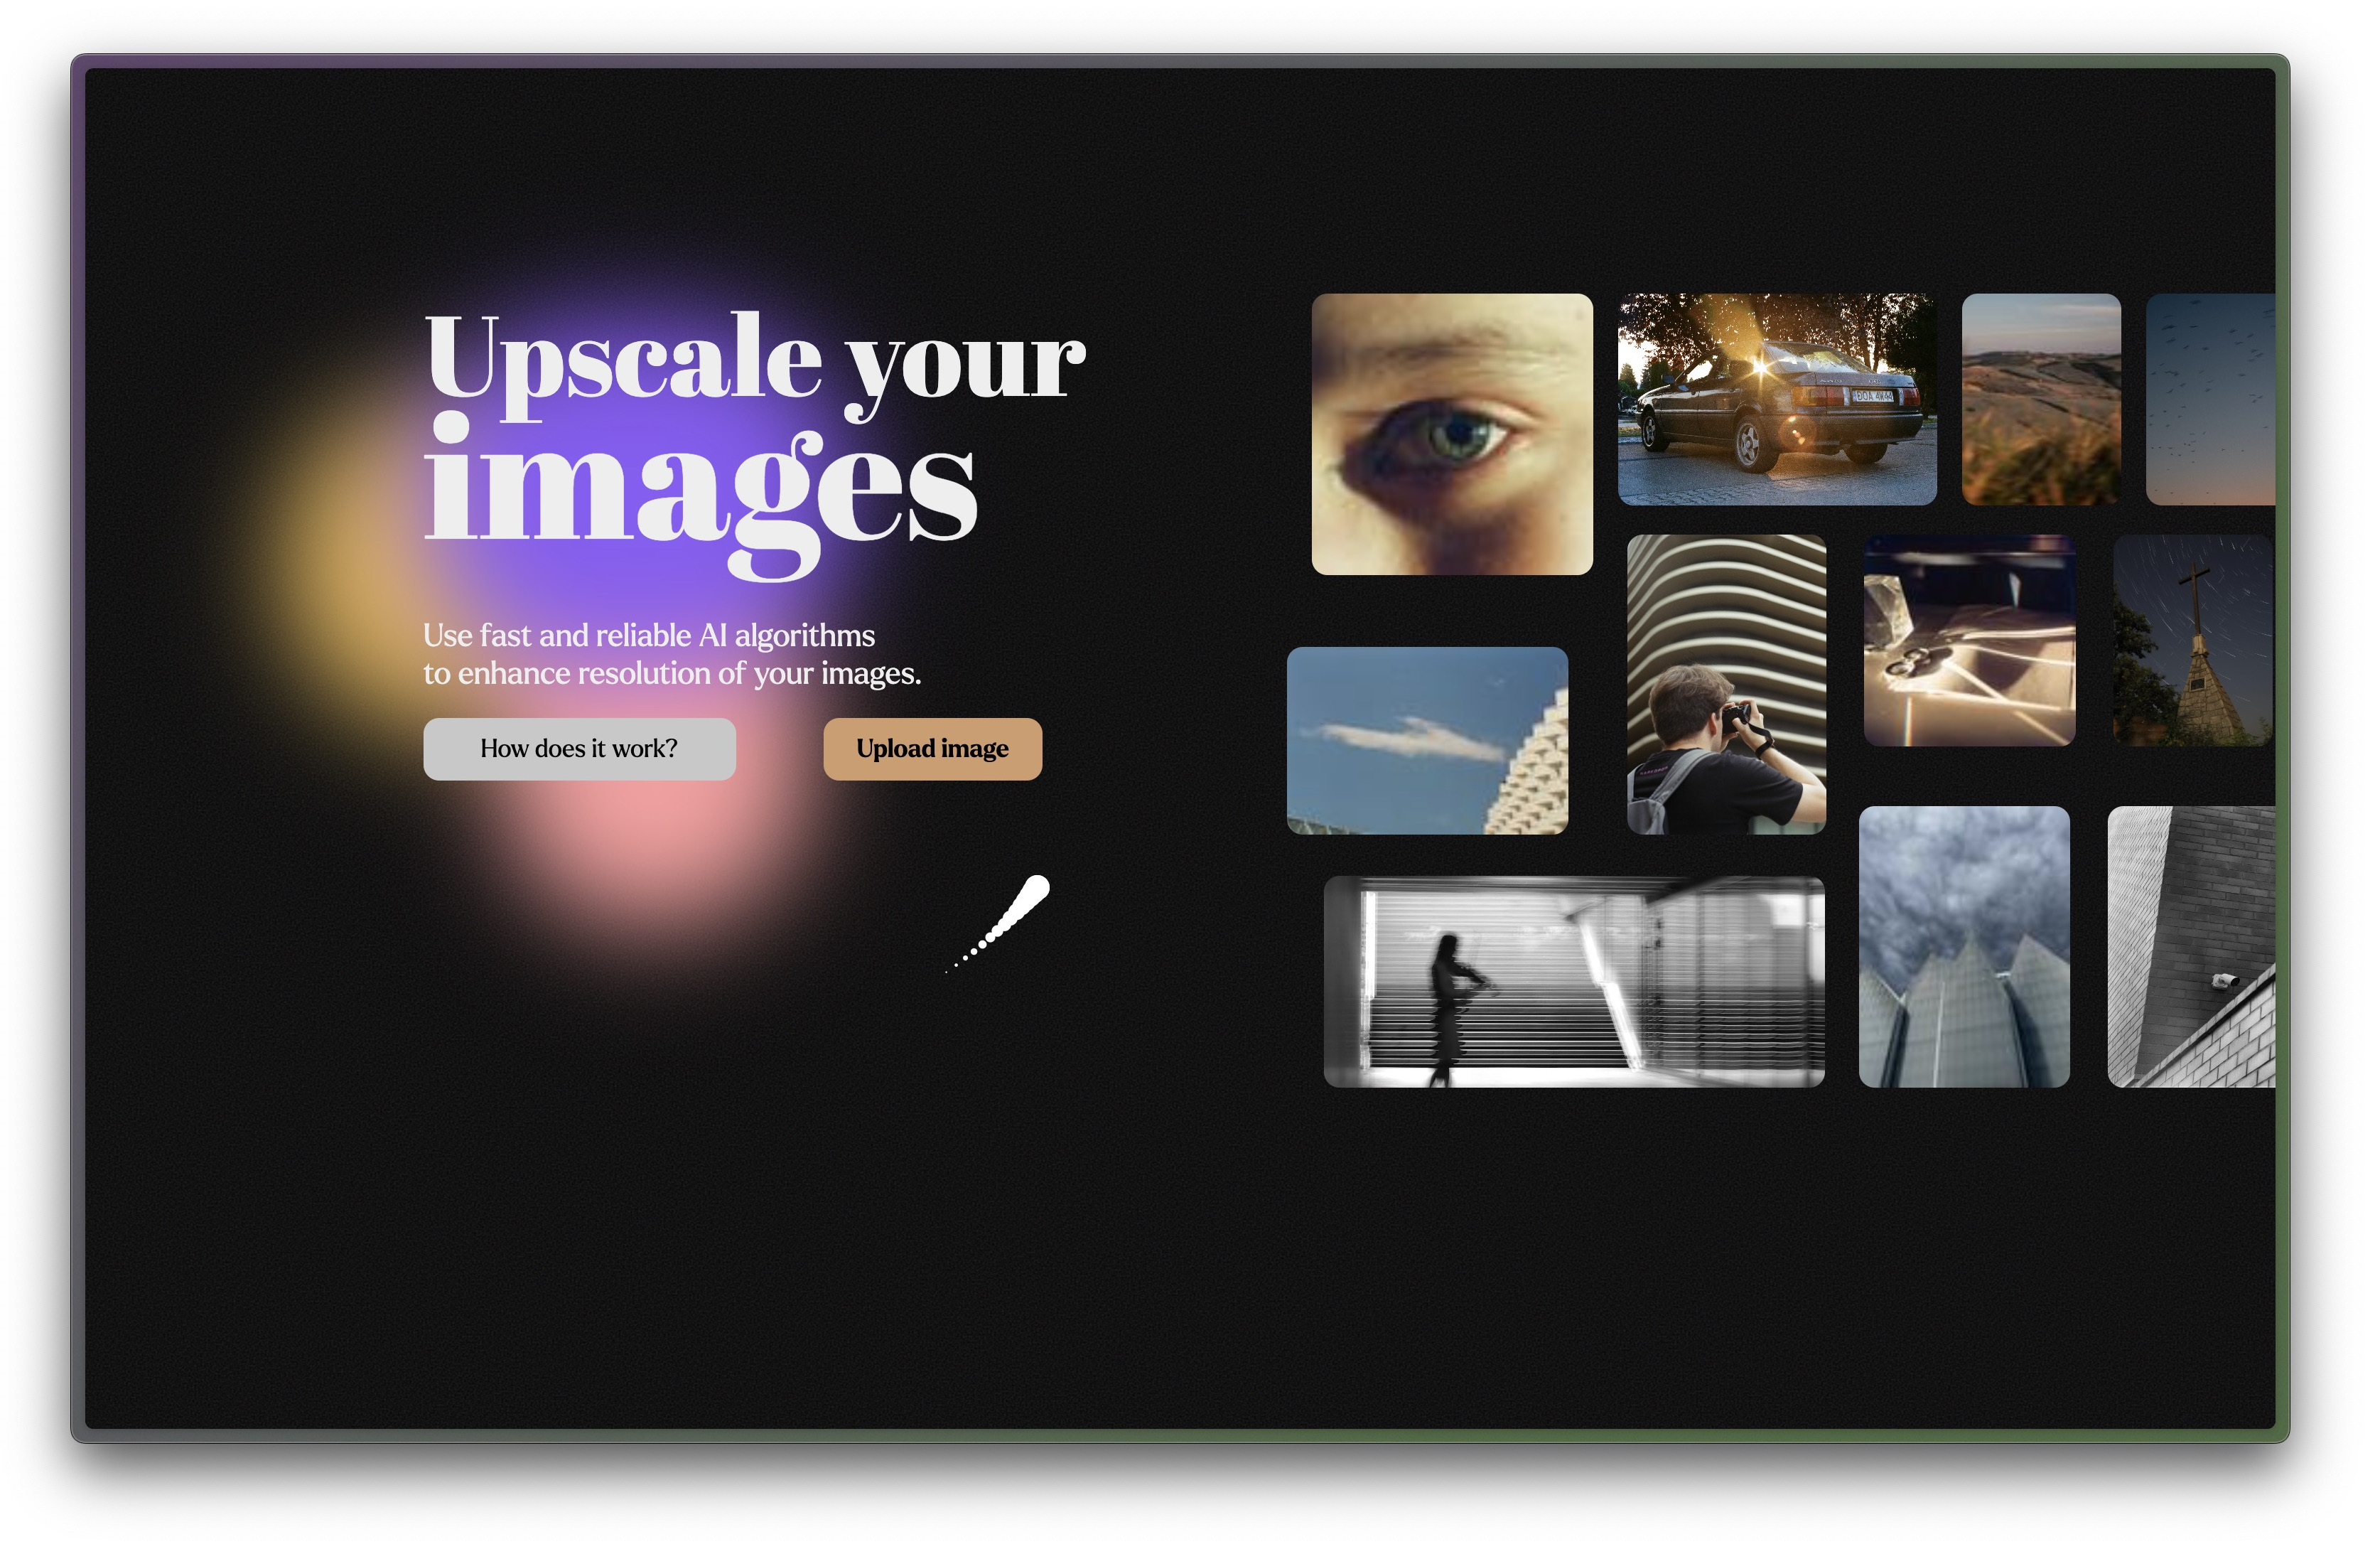
\includegraphics[width=\linewidth]{Rozdziały/06.Aplikacja/Obrazy/kursor-move.jpg}  
    \caption{Widok strony głównej aplikacji}
    \label{fig:image88}
\end{figure}

Widok ten wydaje się drobny i prosty, lecz w rzeczywistości jest rozbudowany. W idei skupić się ma na tym co najważniejsze, czyli na przesłaniu obrazu do powiększenia. Mam sporo pomysłów na ot jak go rozbudować na bazie istniejących interakcji i jakie dodatkowe funkcjonalności można by dodać, ale o tym w rozdziale \ref{sec:plans}.

Widok ten składa się z dwóch części - z tytułu aplikacji oraz przycisków i z obrazów przykładowych [Rys \ref{fig:image88}]. 

W aplikacji znajdziemy dwie czcionki: \textit{Abril Fatface} z Google Fonts \cite{googlefonts} i \textit{Larken} z Adobe Fonts \cite{adobefonts}. Pierwsza z nich jest używana do tytułu aplikacji, a druga do reszty tekstu, przycisków itp.
Niżej na stronie znajdują się dwa przyciski, jeden do przesłania obrazu, a drugi do wyświetlenia informacji o aplikacji. Przycisk do przesłania obrazu jest wyróżniony kolorem, więc od razy zwraca na siebie uwagę, zaś przycisk z informacjami jest w kolorze szarym, więc jest mniej widoczny. Póki co przycisk z informacjami nie ma żadnej funkcjonalności, ale o tym w rozdziale \ref{sec:plans}. 

Prawa część ekranu składa się z obrazów przykładowych, które mają zachęcić użytkownika do przesłania obrazu. Część z nich jest wysokiej rozdzielczości, a część niższej, aby pokazać różnicę między obrazem oryginalnym a przetworzonym przez aplikację. Obrazy te wyłamują się poza siatkę strony, aby nadać stronie dynamiki.

Tło tego widoku, tak jak wspomniałem wcześniej, nawiązuje do szumu na zdjęciach analogowych, dodatkowo składa się z animowanych kształtów które znajdują się za warstwą szumu. Animacja tła jest subtelna i składają się na nią trzy kształty, które poruszają się pomiędzy wyszczególnionymi za pomocą \textit{@keyframes} punktami. W ten sposób uzyskujemy efekt, że kształty poruszają się w sposób płynny i nie przewidywalny.

Kolejnym istotnym elementem na stronie jest kursor. Ma on wbudowane funkcjonalności, które dają szerokie pole do popisu w kwestii interakcji z użytkownikiem. Kursor zmienia swój wygląd w zależności od tego nad jakim elementem znajduje się wskaźnik myszy. Na przykład gdy wskaźnik znajduje się nad przyciskiem, kursor powiększa się i wyświetla się wewnątrz niego ikona. 
Kursor ma kilka stanów do interakcji nad obiektami oznaczonymi klasą \textit{interactable}:

\begin{itemize}
    \item \textbf{Init} - stan początkowy, gdy wskaźnik znajduje się na ekranie, skaluje się od 0 do 1.2 i po osiągnięciu 1.2 zmienia się na stan \textbf{Default}.
    \item \textbf{Default} - stan domyślny, gdy wskaźnik nie znajduje się nad żadnym specjalnym elementem. Warto w tym miejscu dodać, że kursor tak naprawdę składa się z piętnastu elementów, które ciągną cię za miejscem w którym znajduje się wskaźnik. Dzięki temu za każdym ruchem pozostaje ślad, który uprzyjemnia interakcje z aplikacją [Rys \ref{fig:image88}].
    \item \textbf{Hover} - stan nad elementem, gdy wskaźnik znajduje się nad elementem oznaczonym klasą \textit{interactable}, kursor powiększa się i wyświetla się wewnątrz niego ikona w zależności od tego nad czym się znajduje [Rys \ref{fig:image89}, \ref{fig:image90}, \ref{fig:image91}].
    \item \textbf{DragOver} - stan gdy do aplikacji chcemy przeciągnąć obraz, kursor zmienia swój kolor, skaluje się na dużo większy i wyświetla się wewnątrz niego ikona [Rys \ref{fig:image92}].
\end{itemize}

Ikony z których korzystam są z bibliotek \textit{Font Awesome} \cite{fontawesome}, oraz \textit{Heroicons} \cite{heroicons} i są one wykorzystywane w zależności od tego nad jakim elementem znajduje się wskaźnik myszy.
Stan \textbf{DragOver} bardzo uprzyjemnia korzystanie z aplikacji, gdyż kiedy użytkownik tylko przeciągnie obraz nad okno przeglądarki, kursor podąża za nim, więc użytkownik może upuścić obraz w dowolnym miejscu na stronie a obraz się prześle.

\begin{figure}[ht]
    \centering
    \begin{minipage}[t]{0.47\linewidth}
        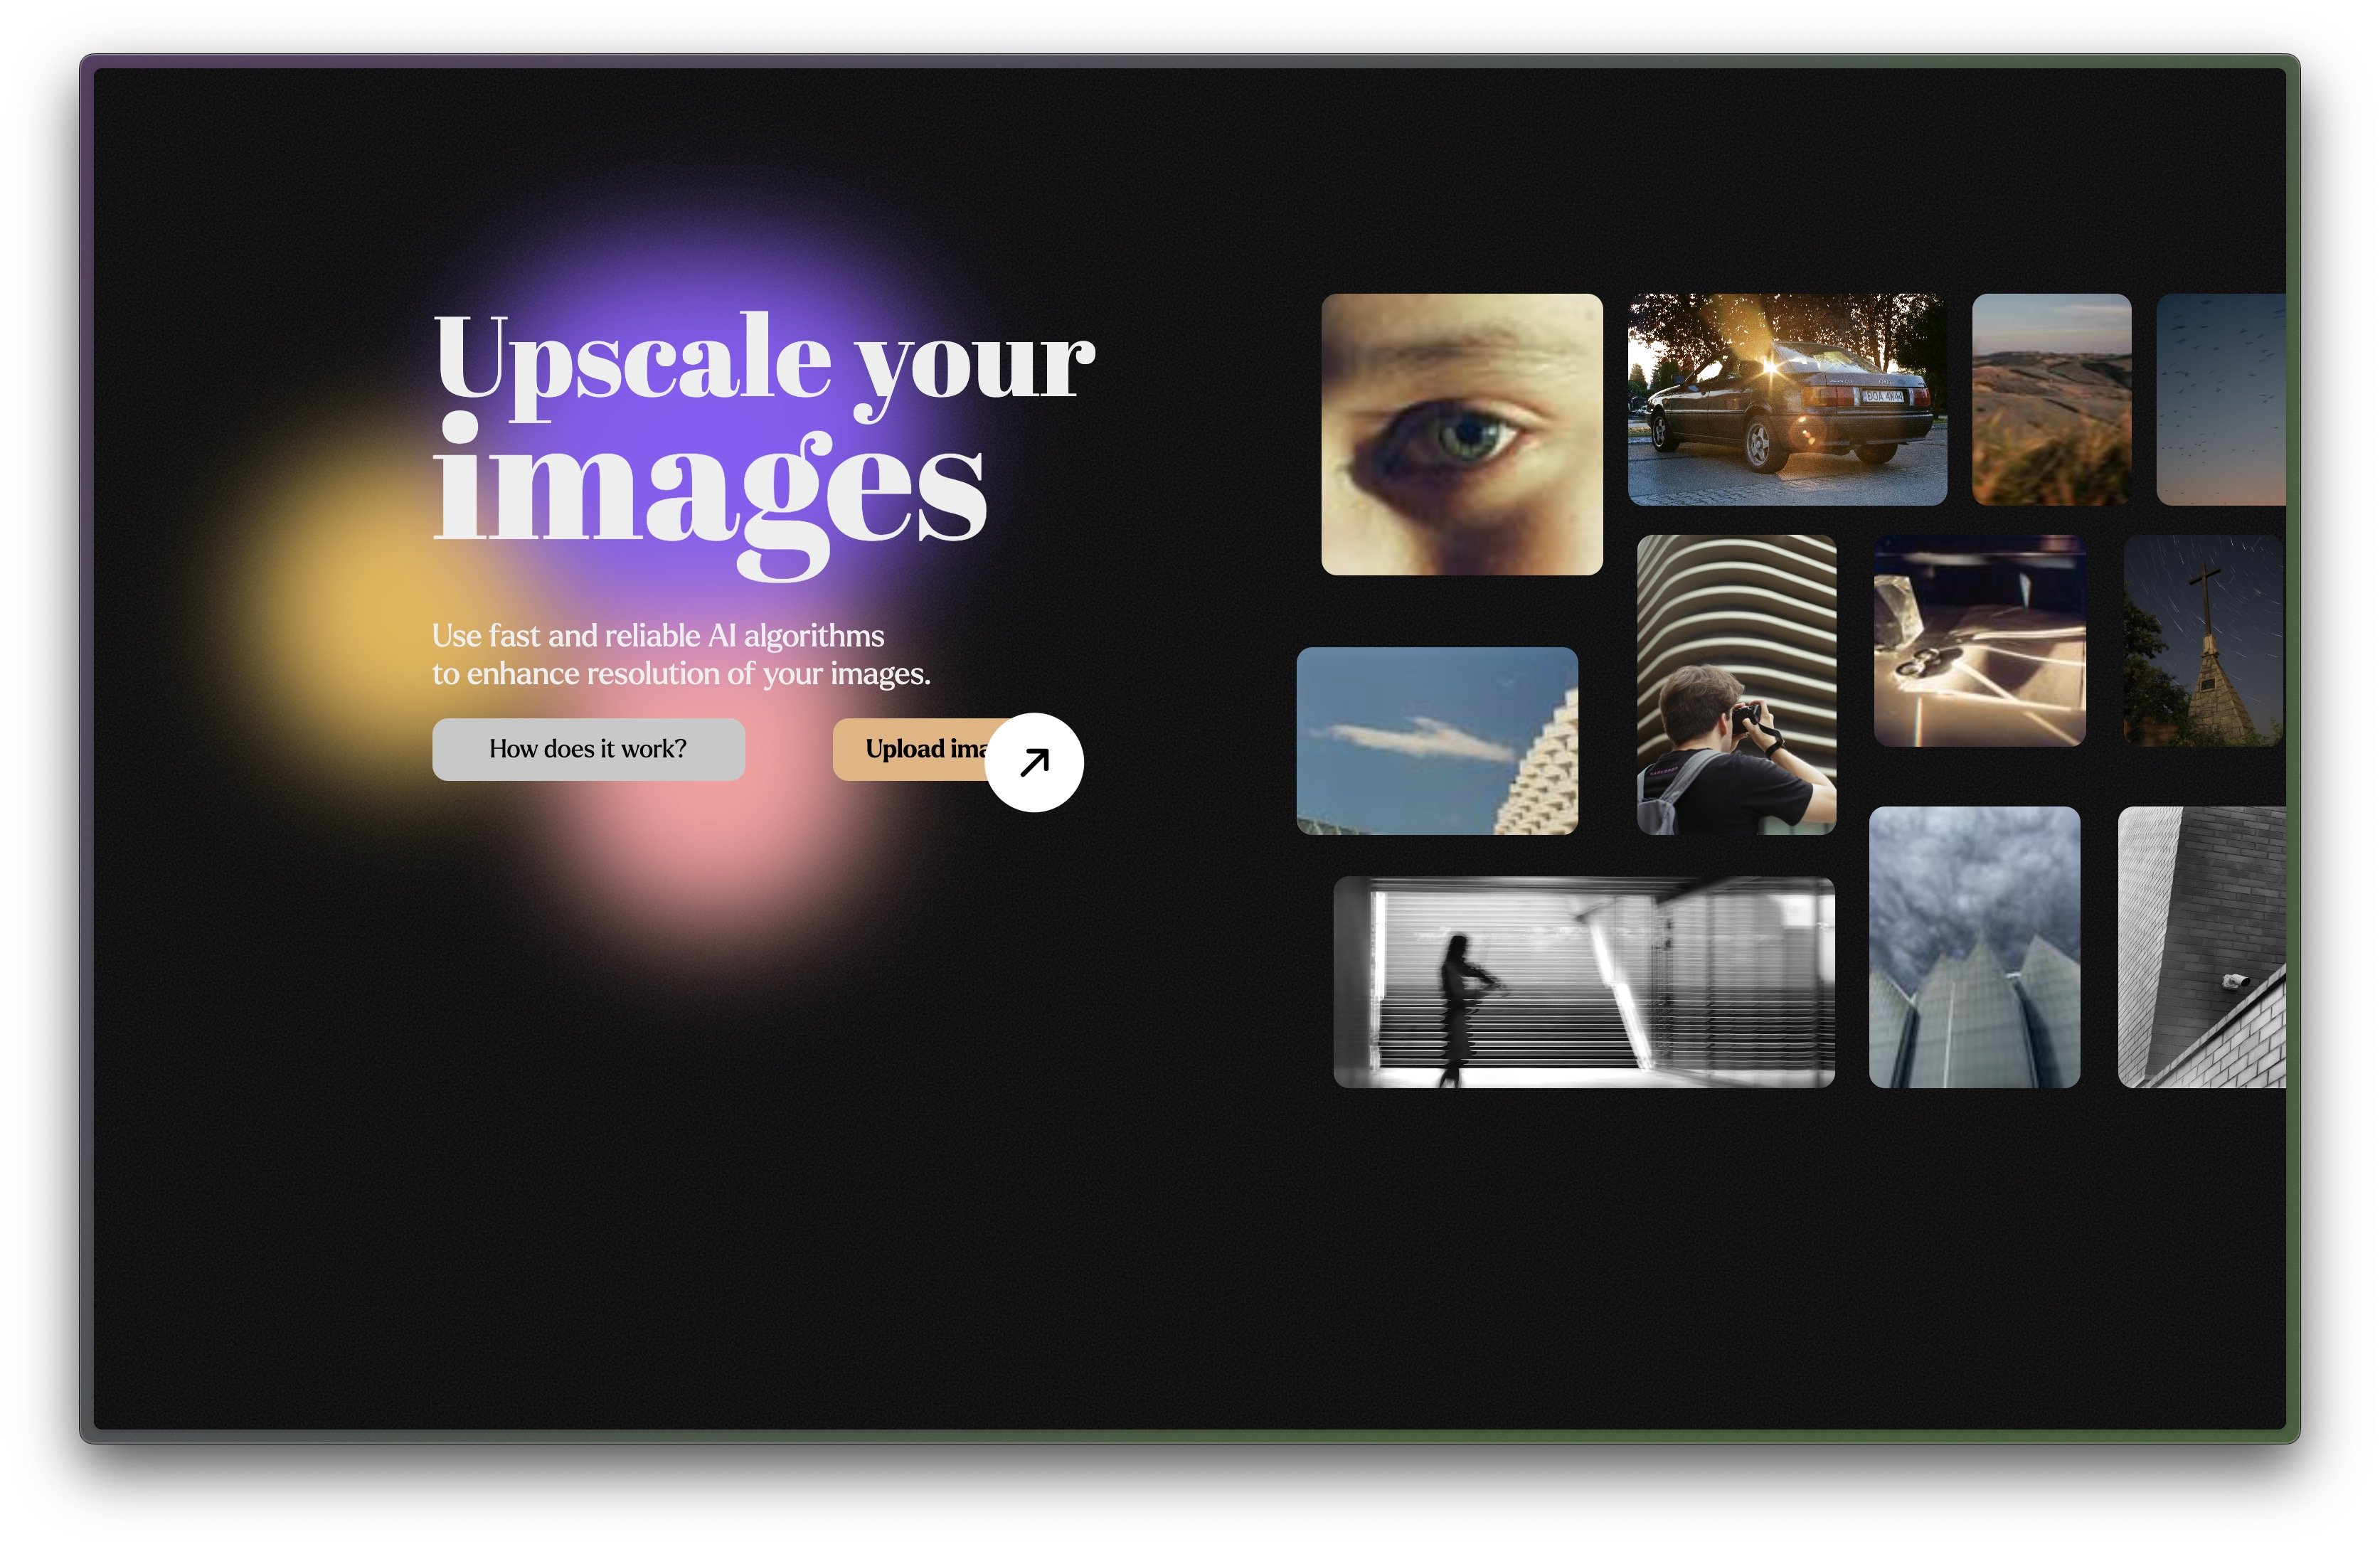
\includegraphics[width=\linewidth]{Rozdziały/06.Aplikacja/Obrazy/kursor-link.jpg}
        \caption{Kursor w stanie Hover (link)}
        \label{fig:image89}
    \end{minipage}
    \hspace{0.5cm}
    \begin{minipage}[t]{0.47\linewidth}
        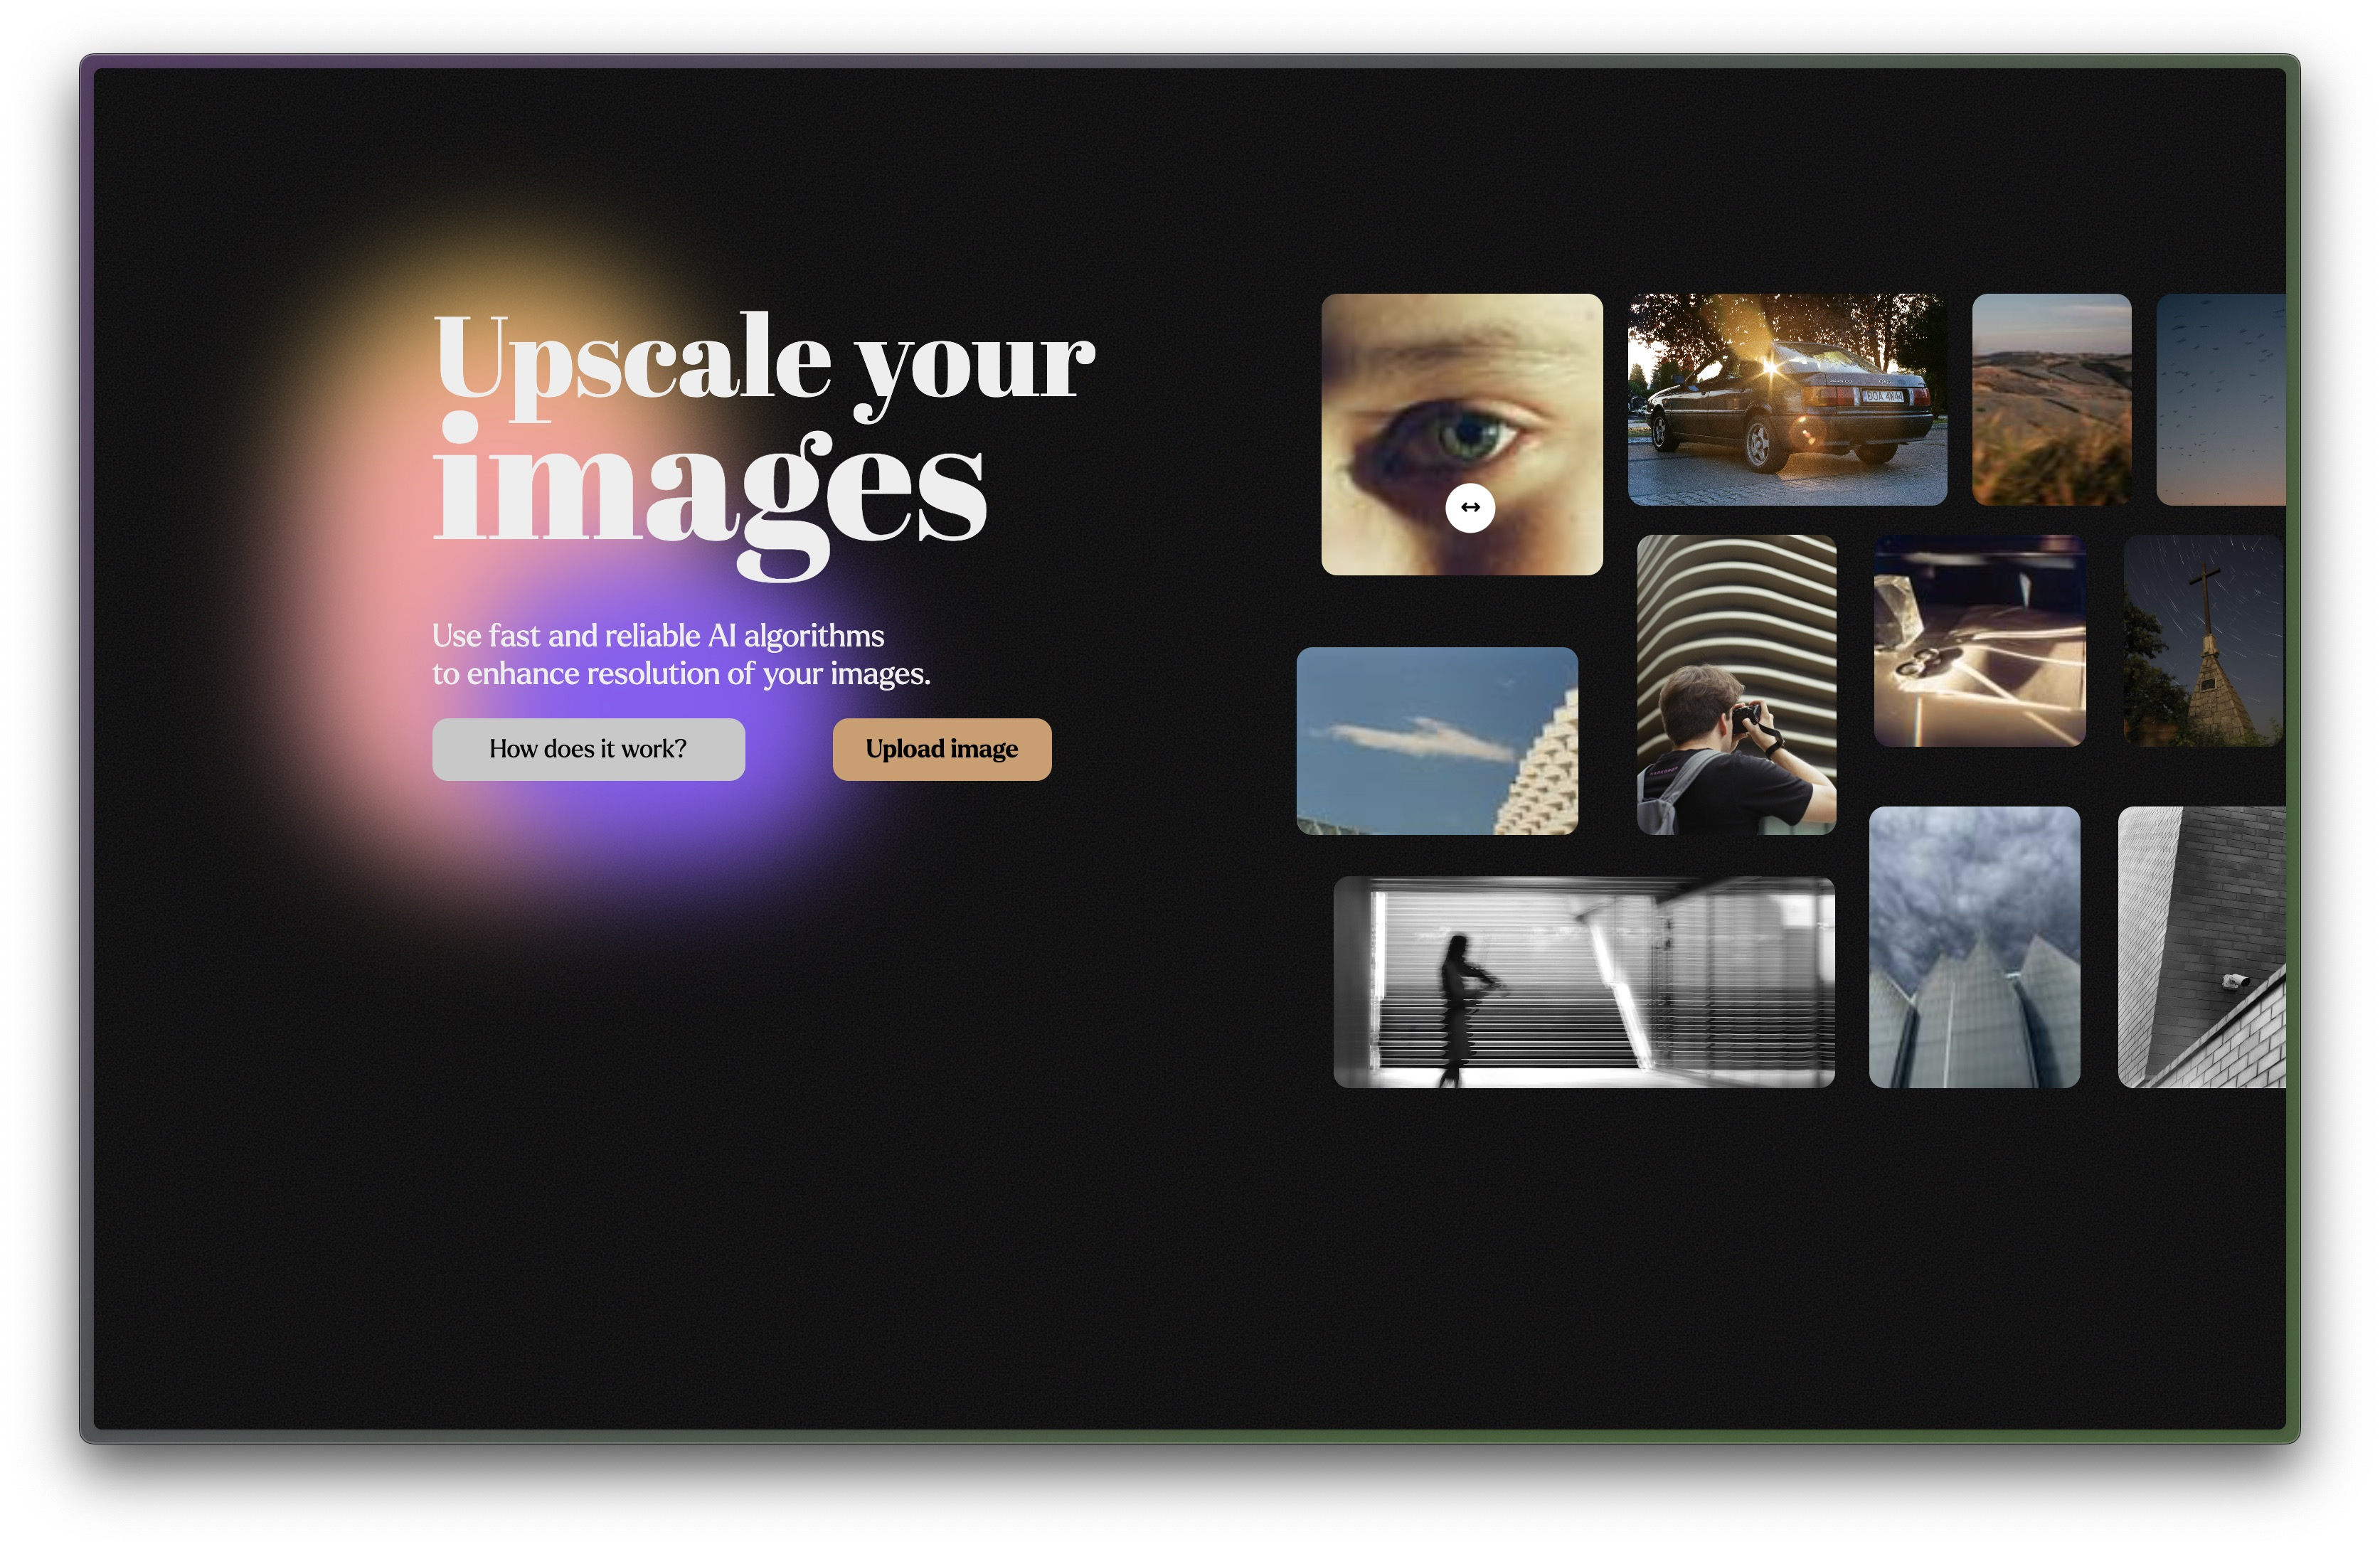
\includegraphics[width=\linewidth]{Rozdziały/06.Aplikacja/Obrazy/kursor-scrabb.jpg}
        \caption{Kursor w stanie Hover (obraz)}
        \label{fig:image90}
    \end{minipage}
\end{figure}

\begin{figure}[ht]
    \centering
    \begin{minipage}[t]{0.47\linewidth}
        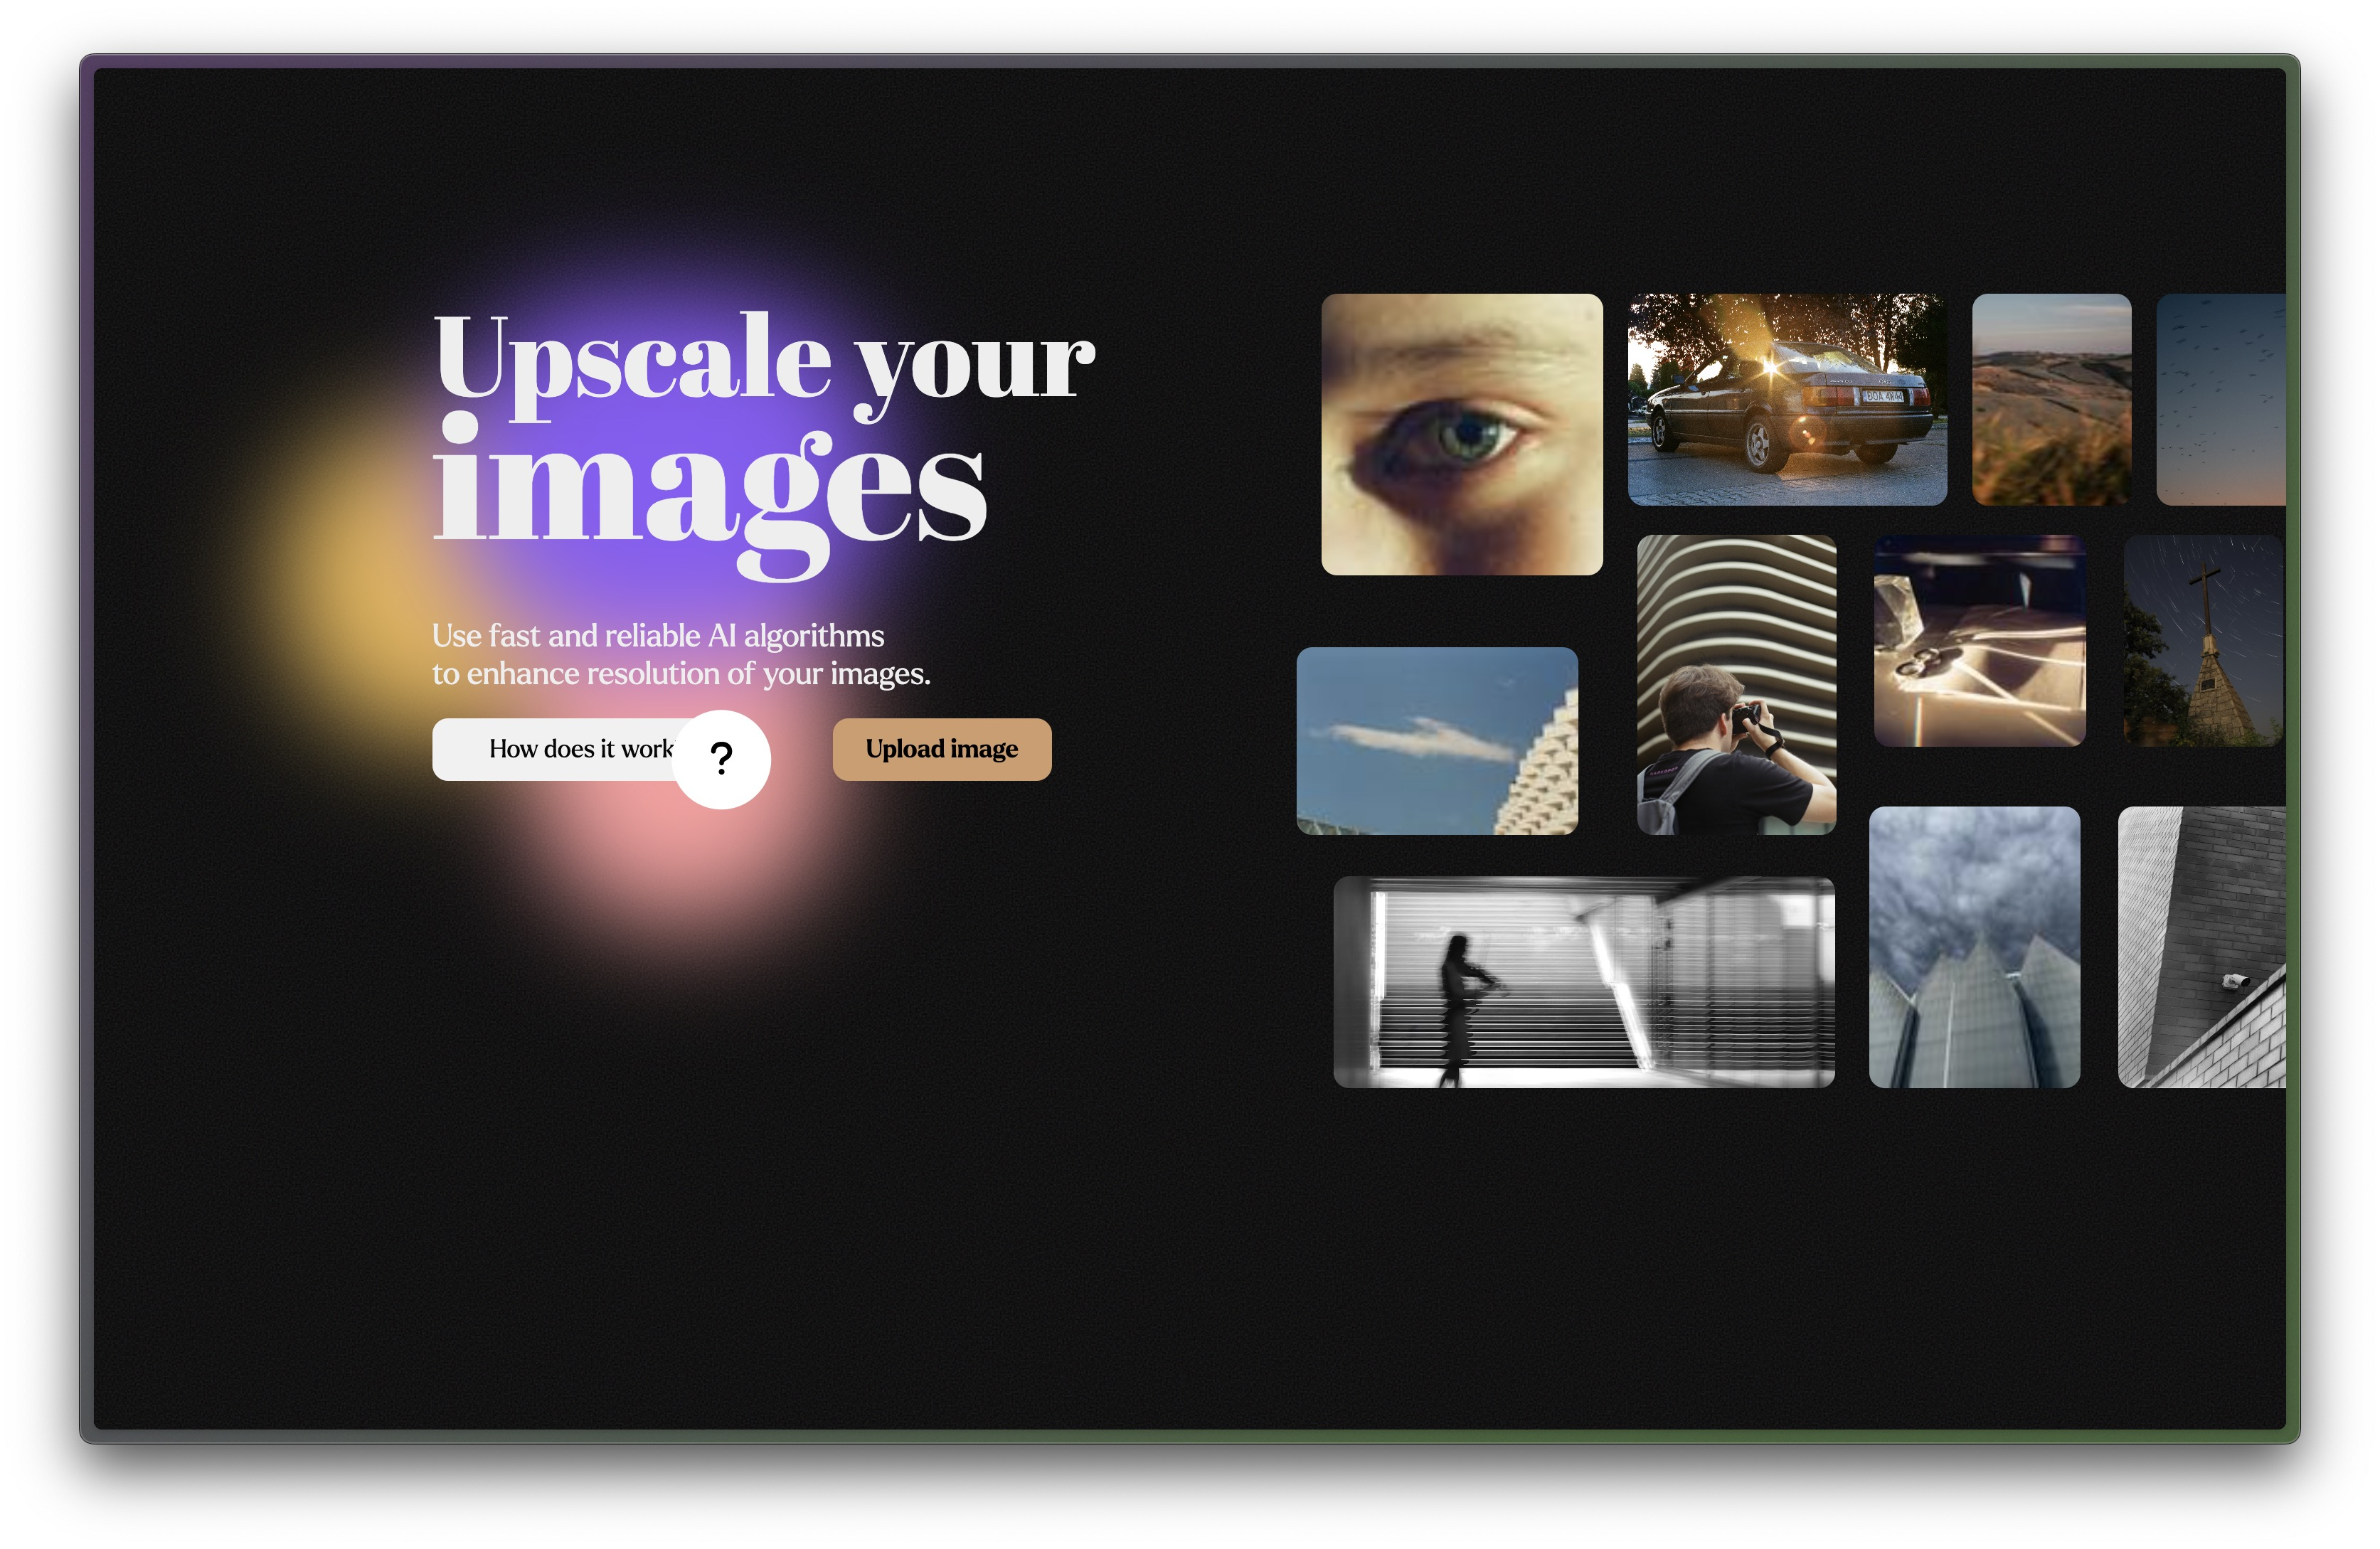
\includegraphics[width=\linewidth]{Rozdziały/06.Aplikacja/Obrazy/kursor-question.jpg}
        \caption{Kursor w stanie Hover (przycisk)}
        \label{fig:image91}
    \end{minipage}
    \hspace{0.5cm}
    \begin{minipage}[t]{0.47\linewidth}
        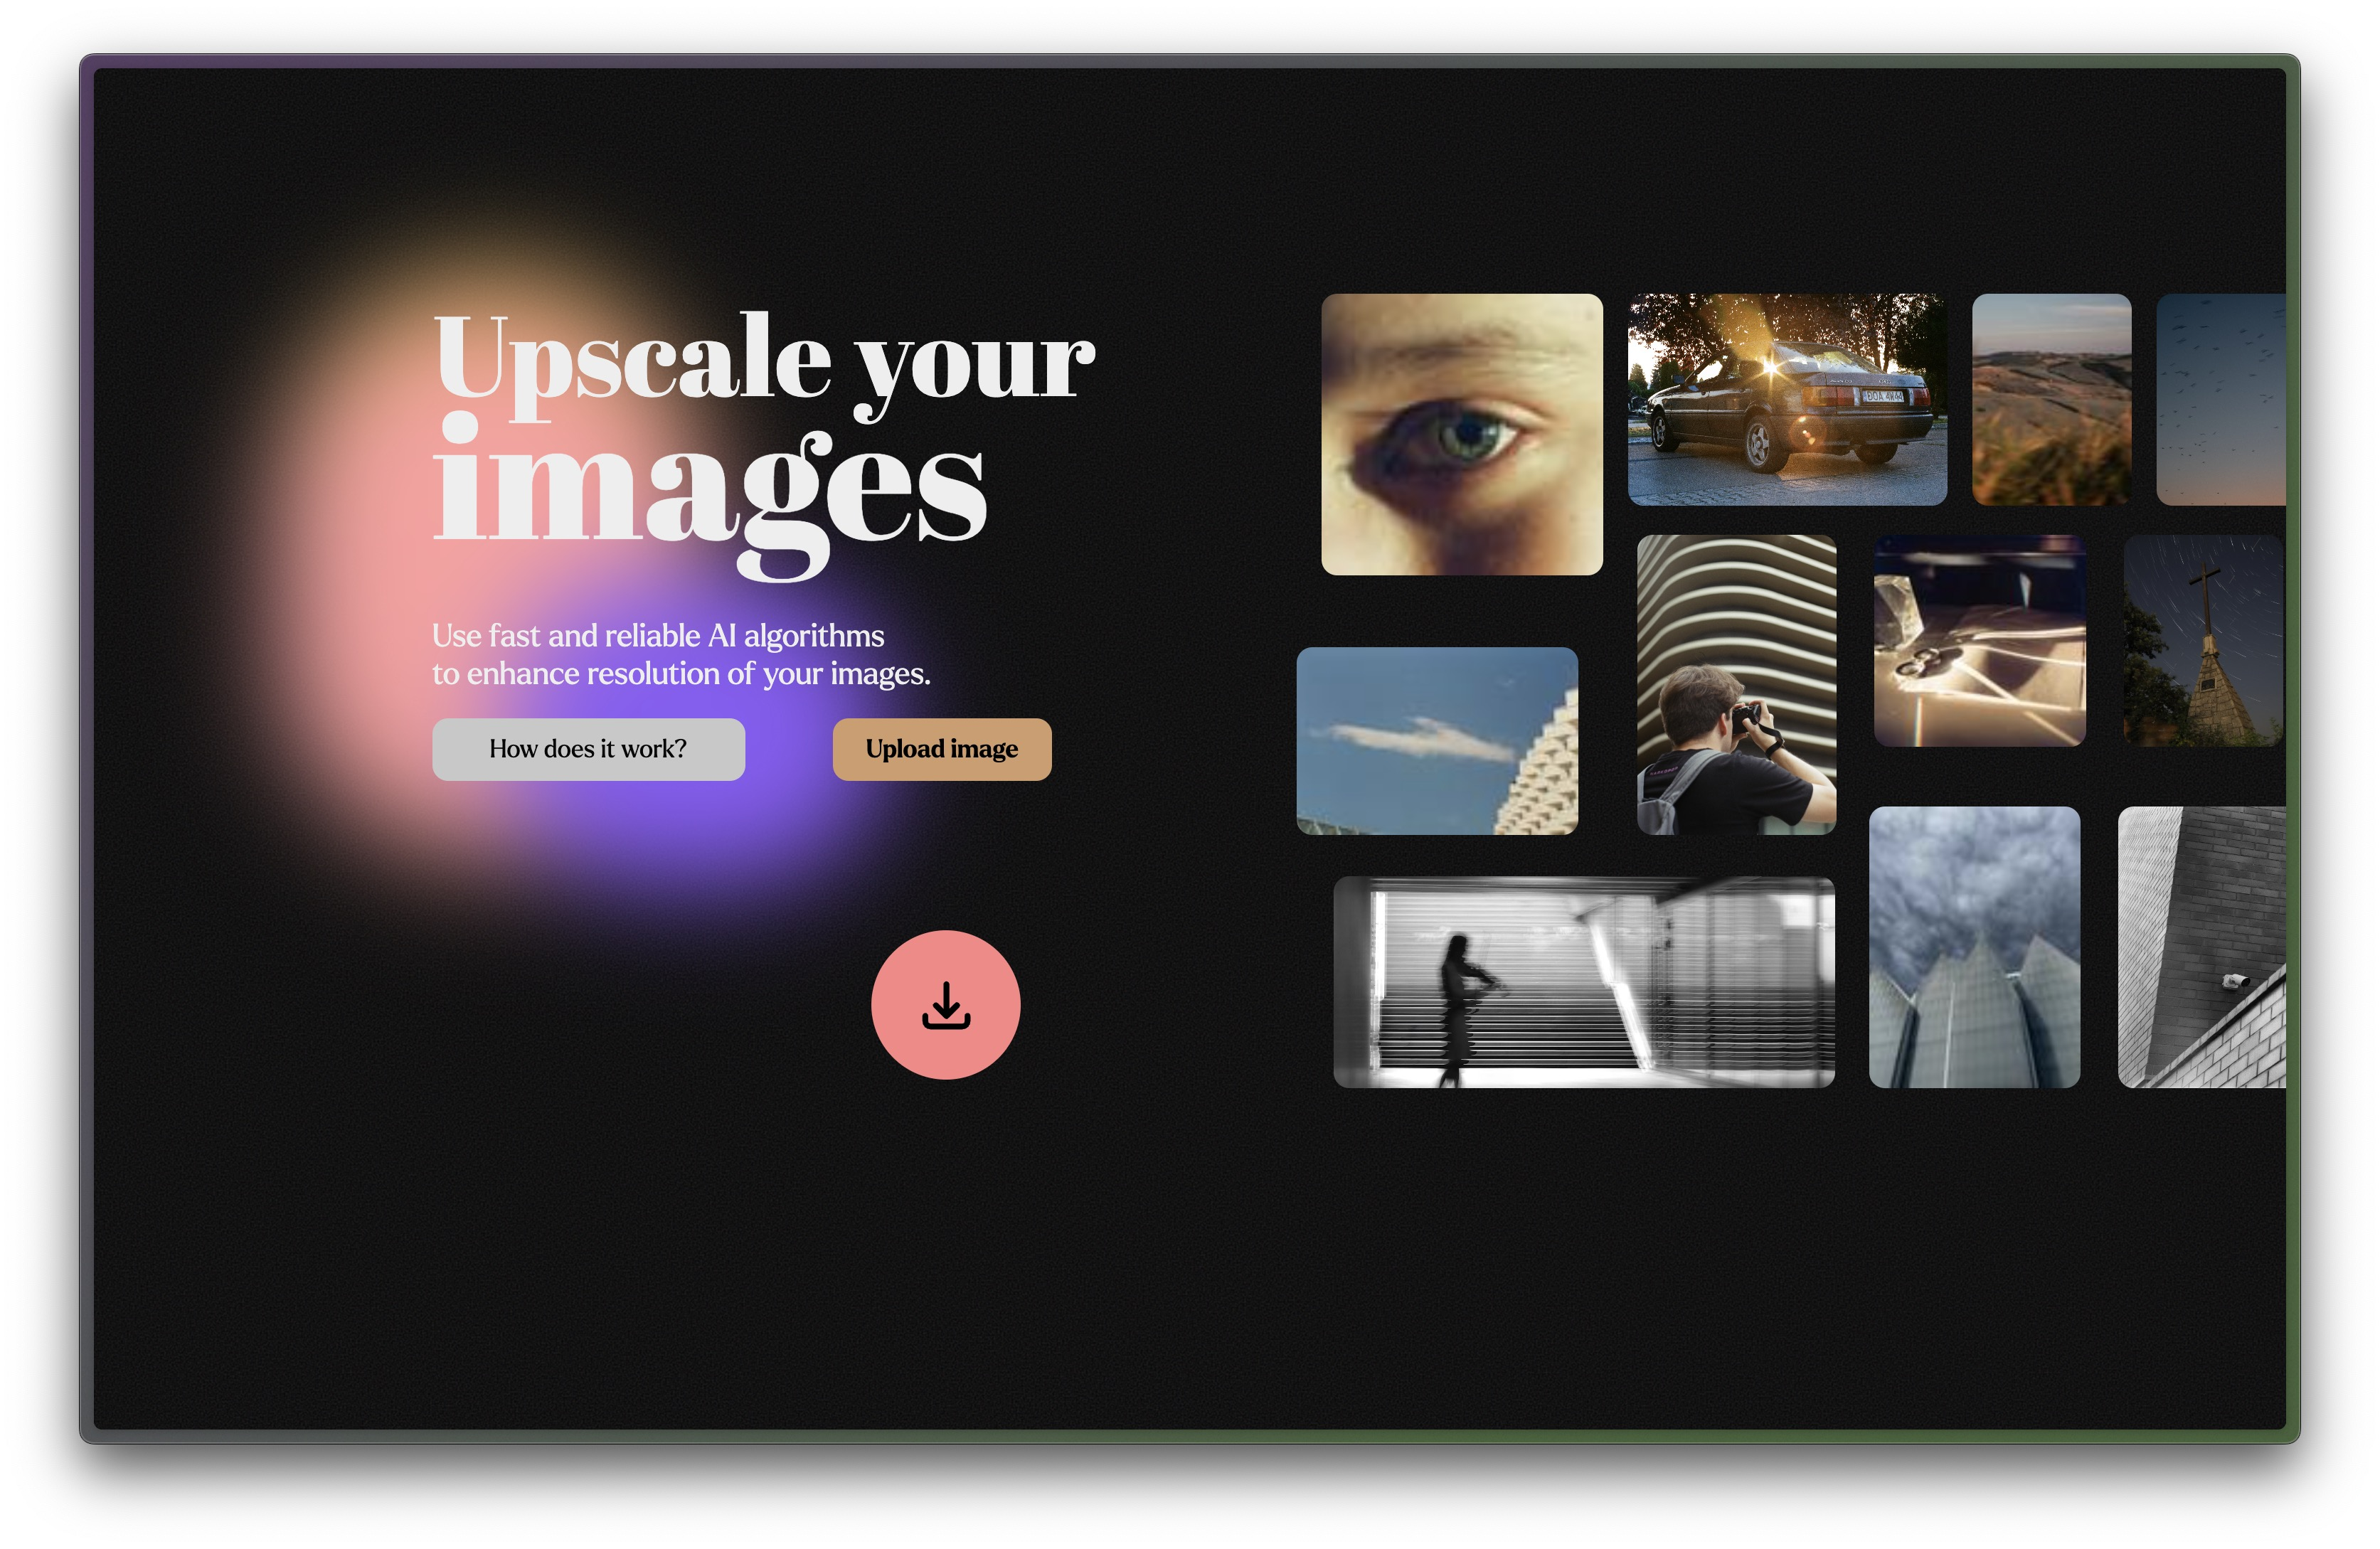
\includegraphics[width=\linewidth]{Rozdziały/06.Aplikacja/Obrazy/kurssor-upload.jpg}
        \caption{Kursor w stanie DragOver}
        \label{fig:image92}
    \end{minipage}
\end{figure}


Gdy obraz zostaje upuszczony, uruchamiana jest funkcja, która odpowiada za sprawdzenie ile plików zostało przesłanych, czy jest to obraz jest wspieranego typu i jeśli wszystko się zgadza wysyła obraz do serwera Backend. Wtedy oczekuje odpowiedzi z Backendu, jeśli wszystko się powiedzie, czyli obraz zostanie zapisany w bazie danych, to Frontend otrzymuje ID obrazka i router zmienia adres na "upload-image/:id". 



\subsection*{Widok z porównaniem wyników powiększenia obrazów}

Drugi widok w aplikacji jest dużo ważniejszy i bardziej rozbudowany, gdyż odpowiada za porównanie wyników powiększenia obrazów. Widok ten składa się z dwóch części - z wybranego obrazu który jest wyświetlony, oraz z menu bocznego [Rys \ref{fig:image93}].

Największą część ekranu zajmuje aktualnie wyświetlany obraz wynikowy, ale tak naprawdę najważniejsze w tym widoku jest menu boczne. Widać na nim podstawowe informacje o obrazie takie jak miniatura, nazwa, nowa (powiększona) rozdzielczość, przycisk do pobrania obrazu oraz co najważniejsze - kafelki z przetworzonymi obrazami. Kafelki te są interaktywne, więc po kliknięciu w nie, obraz jest wyświetlany w głównym obszarze widoku, ale co jeszcze ważniejsze - przybliżony na kafelku fragment obrazu jest fragmentem, który jest pod kursorem myszy. 

Kursor w tym widoku wizualnie jest bardziej złożony, zawiera ikonę sugerującą że działa jak lupa, która wyświetla się w stanie domyślnym. Oprócz tego w lewą górną stronę rozciąga się "szkło" lupy które jest animowane i porusza się wraz z kursorem. 
Dodatkowo zaimplementowałem obsługę scorlla oraz przycisków "+" i "-", która pozwala na przybliżenie i oddalenie obrazu lupy, co sprawia że całe narzędzie jest intuicyjne [Rys \ref{fig:image94}]. Pasek postępu widoczny jest jedynie gdy użytkownik przybliża lub oddala obraz. 

\begin{figure}[H]
    \centering
    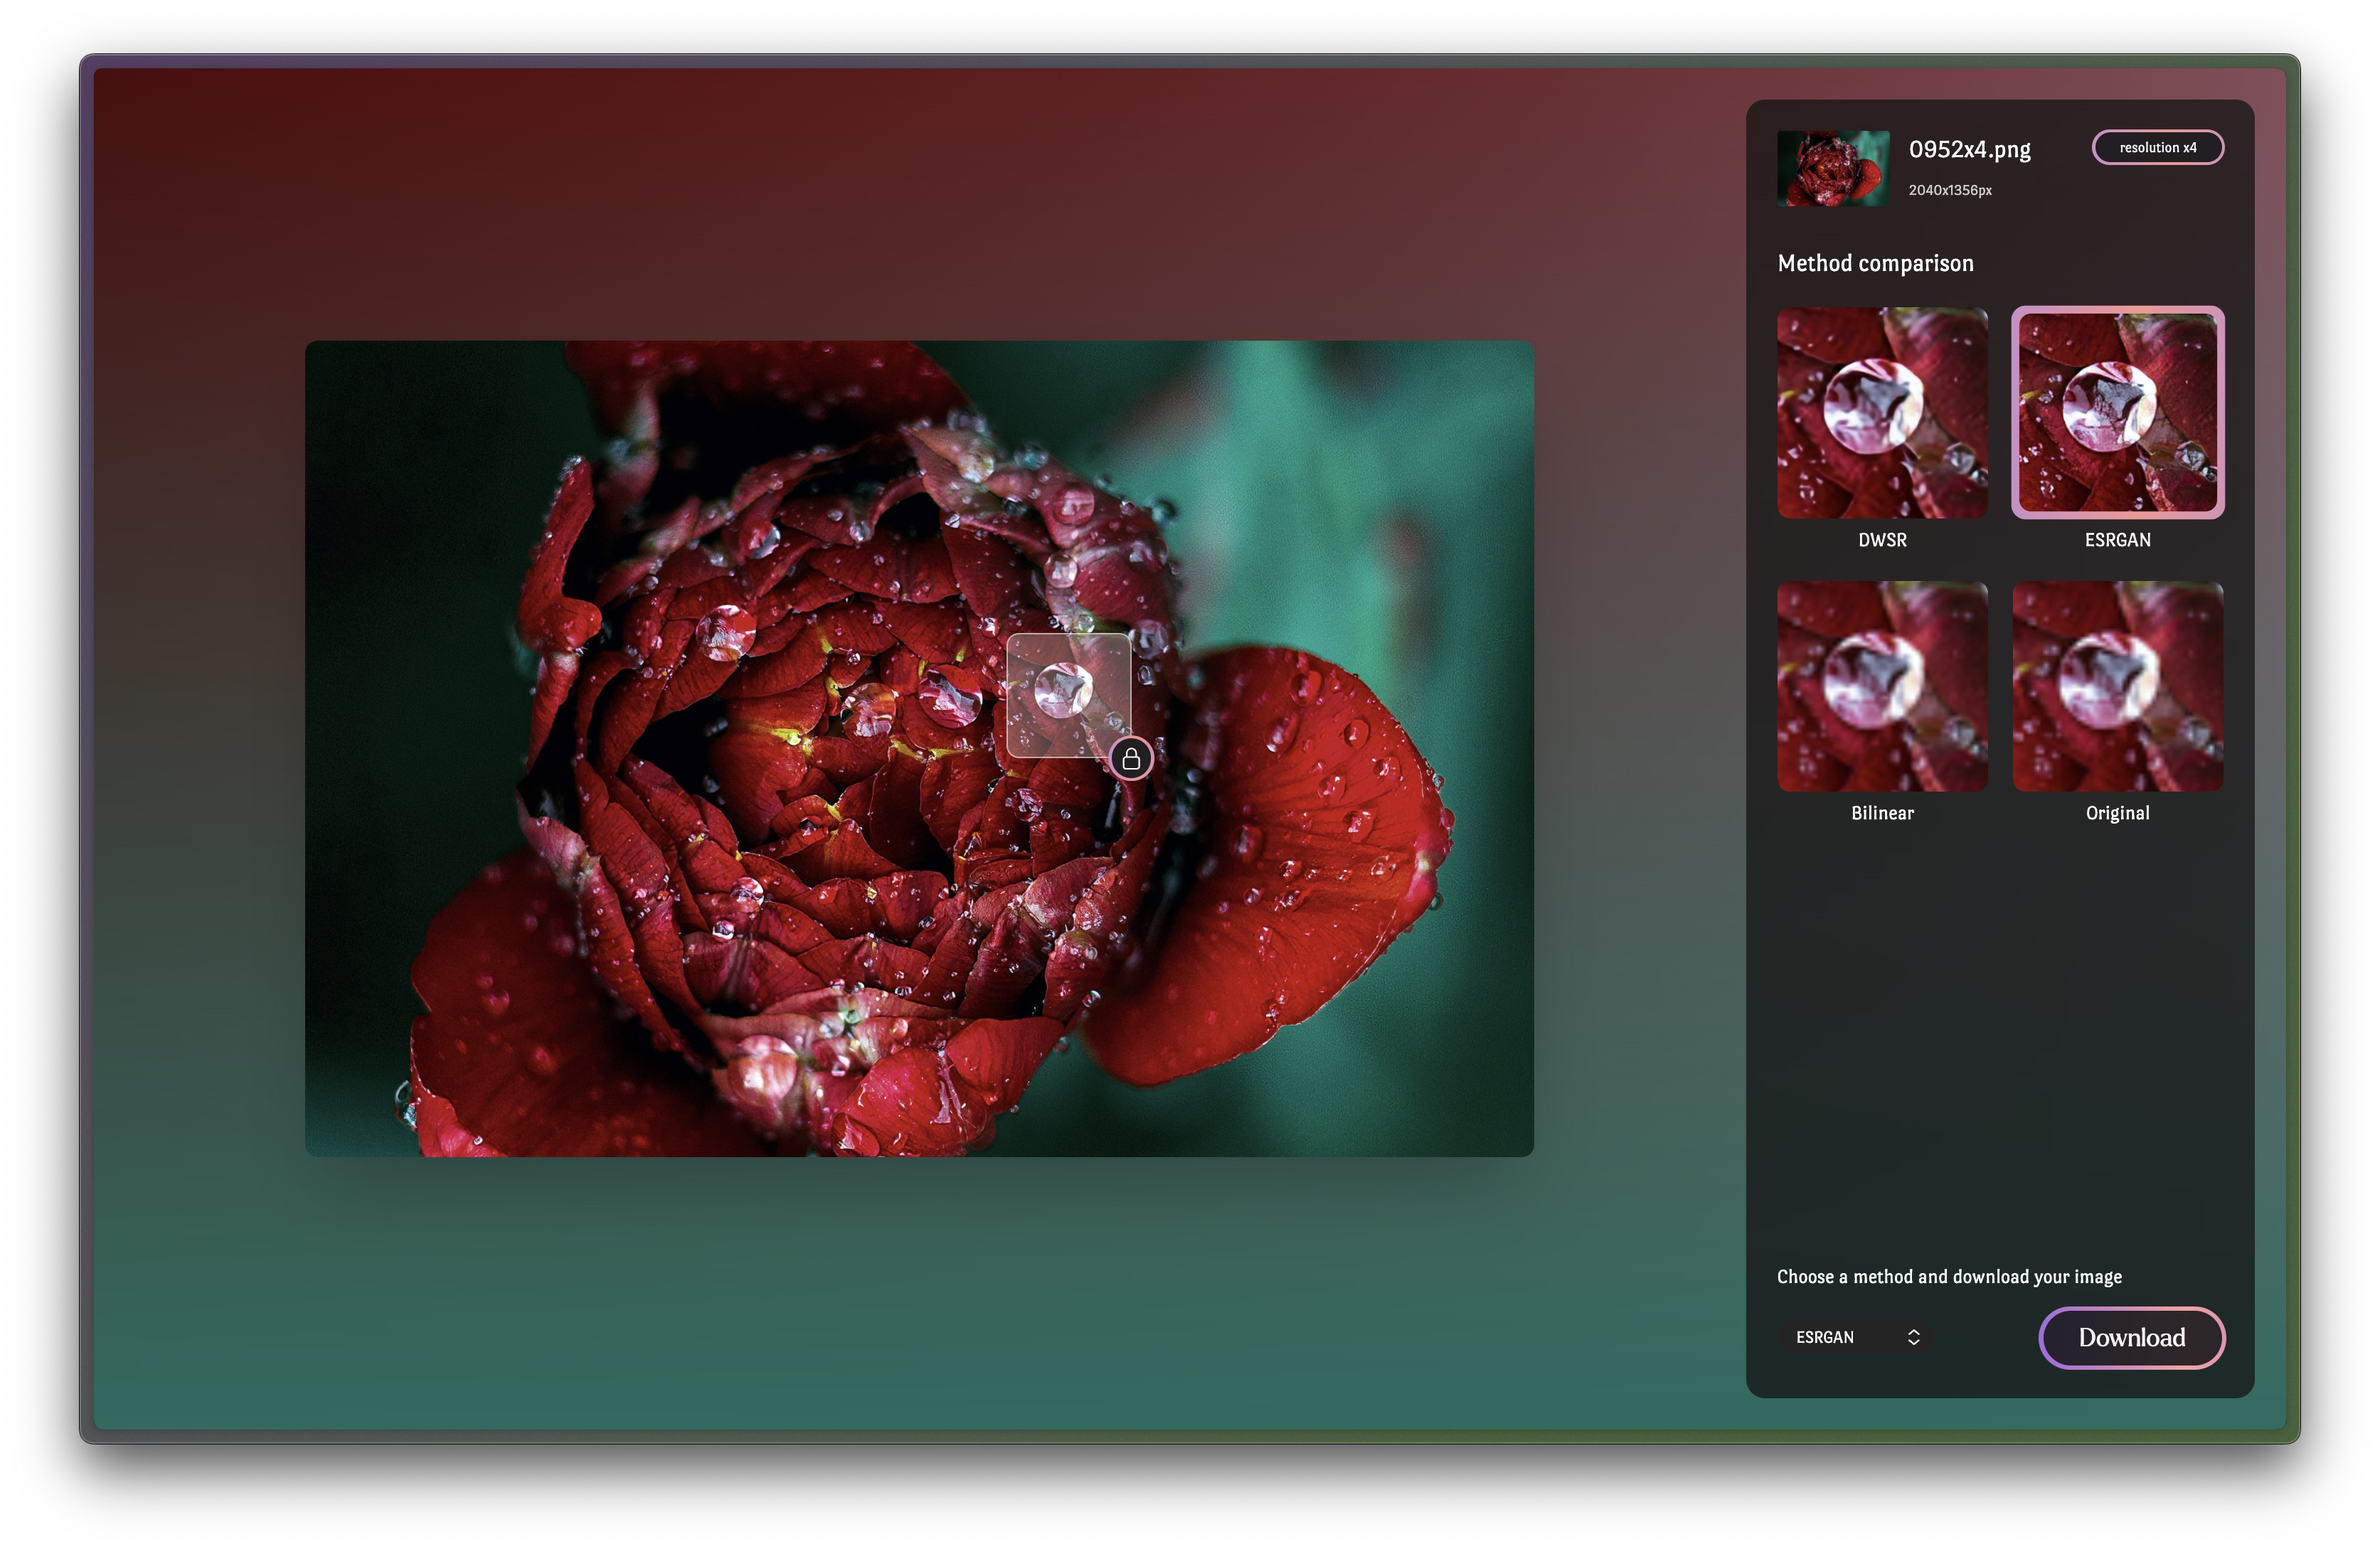
\includegraphics[width=\linewidth]{Rozdziały/06.Aplikacja/Obrazy/display4.jpg}  
    \caption{Widok z porównaniem wyników algorytmów (obraz z \cite{guo2017deep})}
    \label{fig:image93}
\end{figure}

\begin{figure}[H]
    \centering
    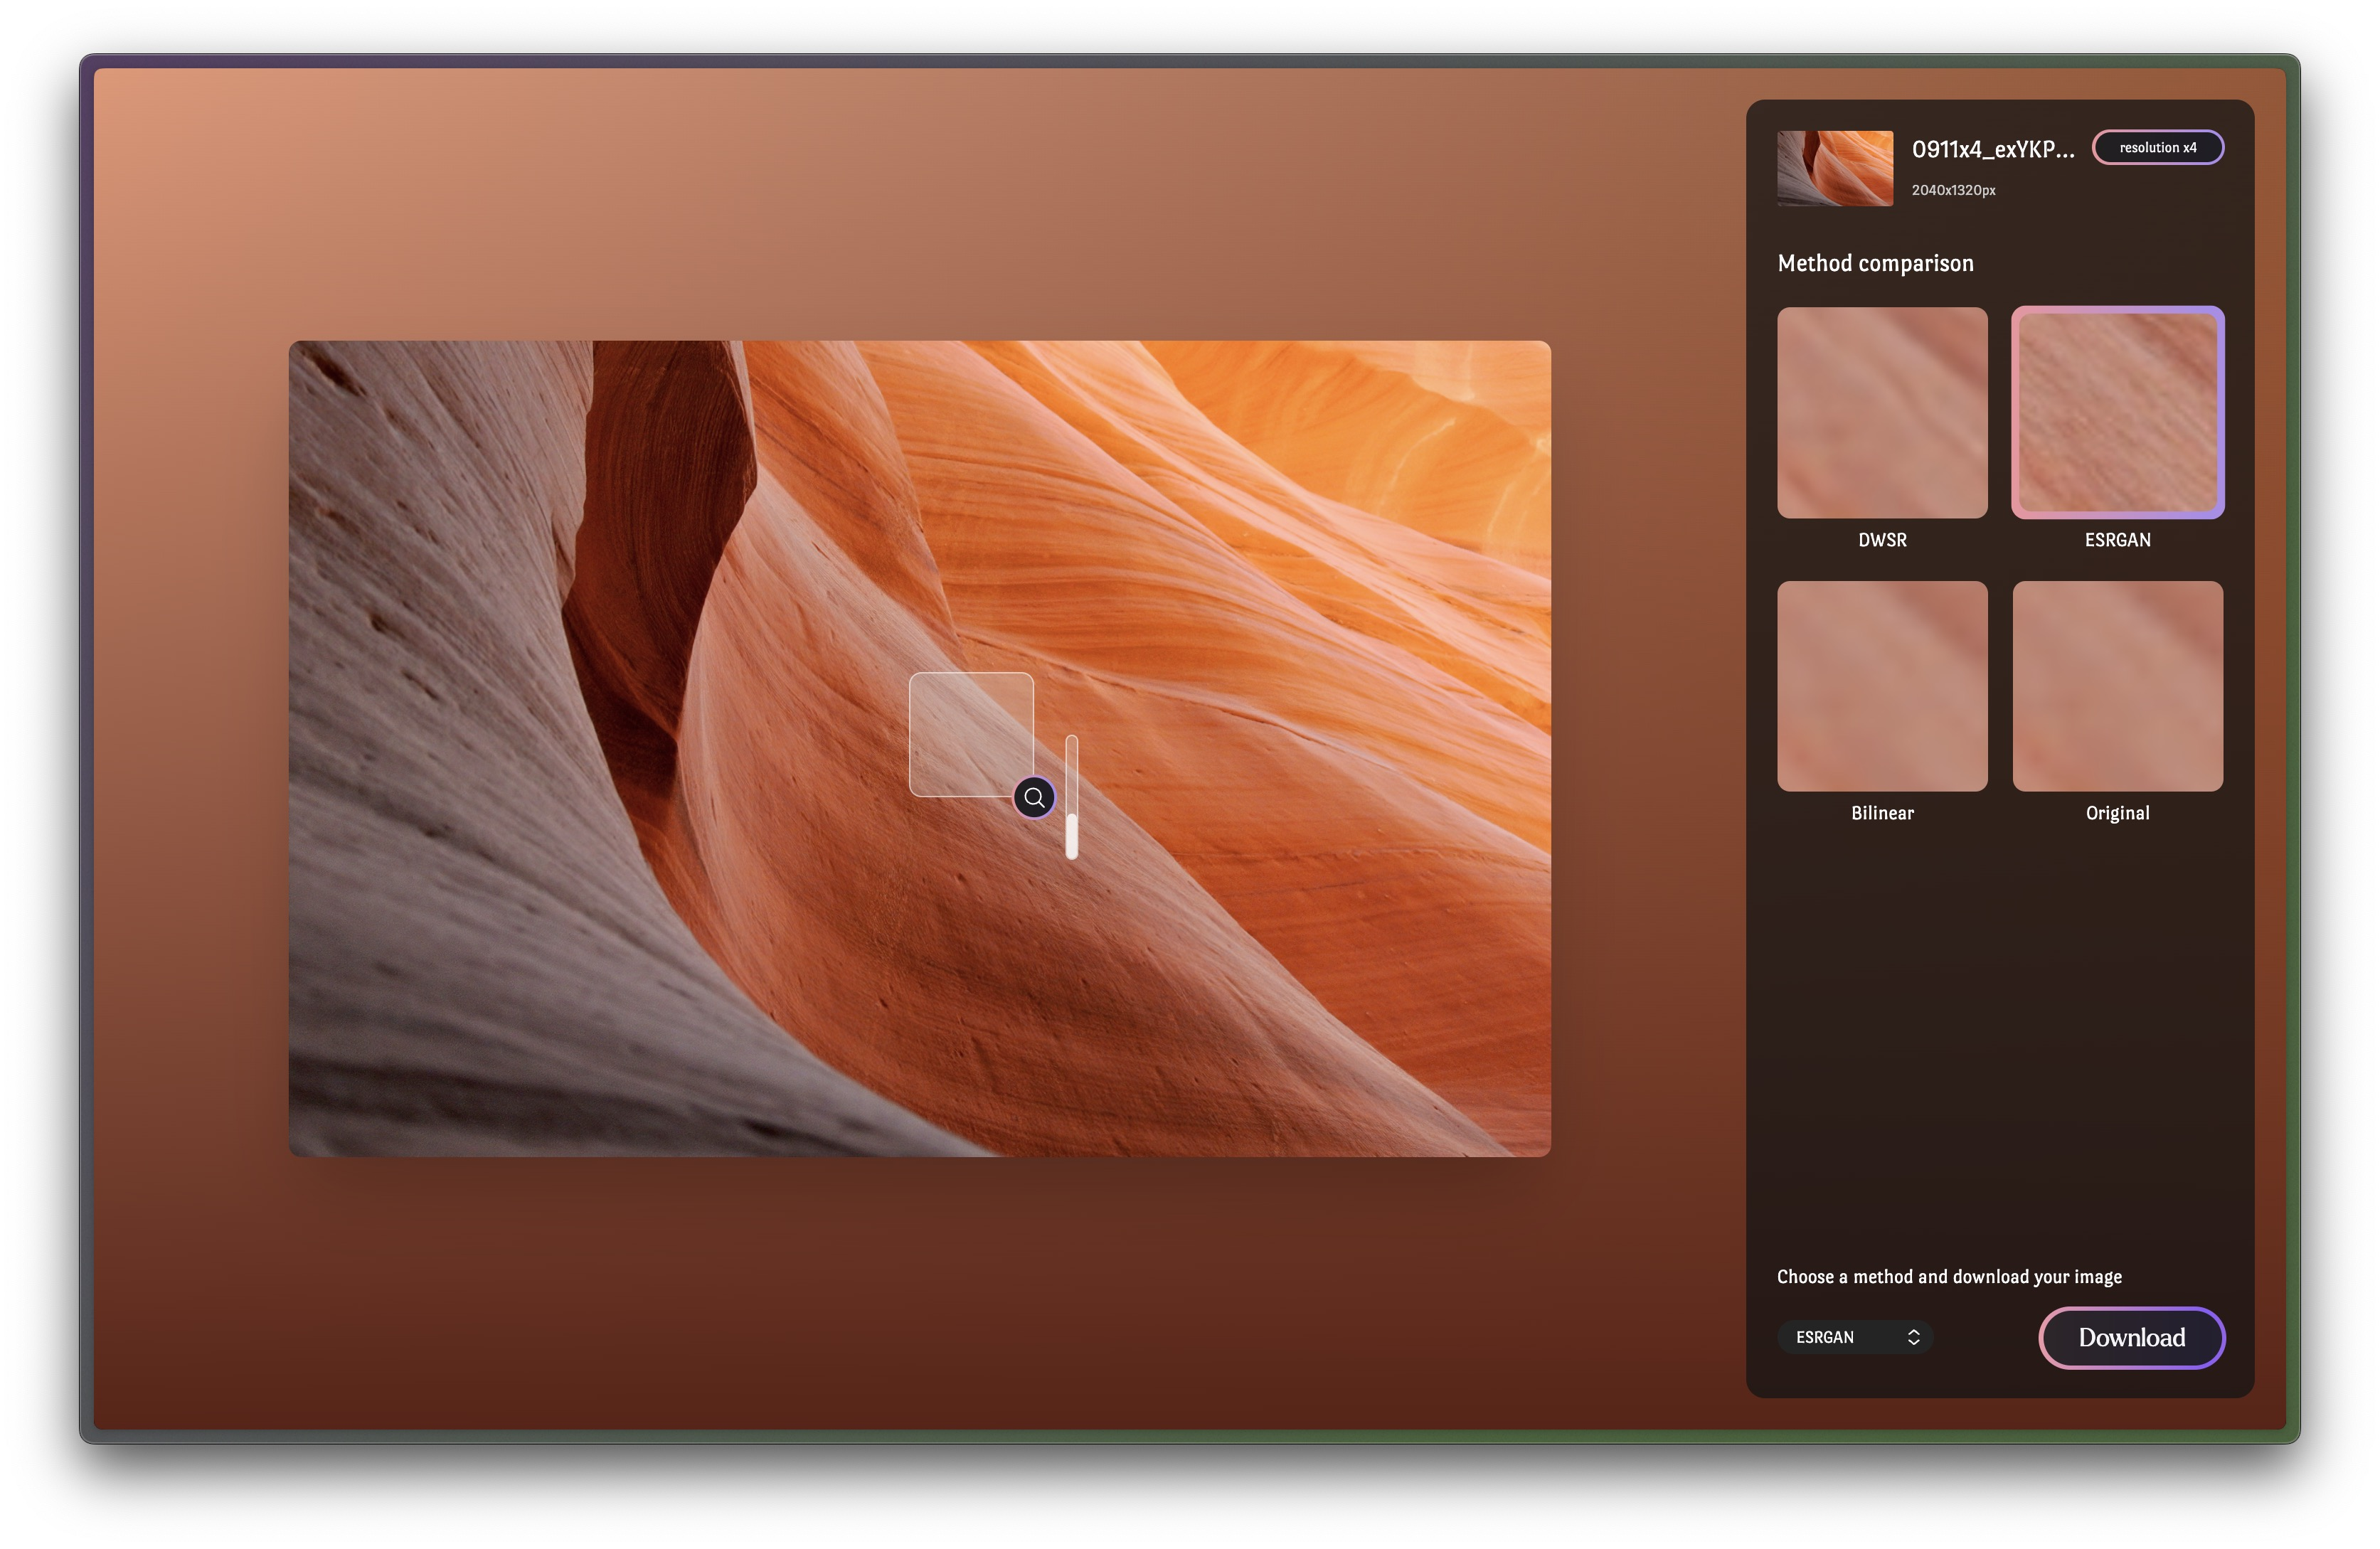
\includegraphics[width=\linewidth]{Rozdziały/06.Aplikacja/Obrazy/display1.jpg}  
    \caption{Widok z porównaniem wyników algorytmów (obraz z \cite{guo2017deep})}
    \label{fig:image94}
\end{figure}

\newpage
Kursor ma też opcję blokady w miejscu, która jest aktywowana po przytrzymaniu klawisza spacji lub po kliknięciu myszą. Sprawia ona że kursor nie porusza się wraz z myszą, więc użytkownik może swobodnie poruszać się po aplikacji. W stanie blokady na kursorze wyświetla się ikona z kłódką, która sugeruje blokadę kursora

Tłem widoku jest gradient kolorów dominujących na obrazie. Kolory te są wyliczane przez algorytm K-średnich na Backendzie i zapisywane w bazie danych, dzięki temu Frontend może je wykorzystać. 

\begin{lstlisting}[language=TypeScript, caption=Wyznaczanie gradientów z kolorów dominujących., label={lst:colors}]
const generateGradientStyles = (colors: string[]) => {
    const angles = ['45deg', '135deg', '-45deg', '90deg', '0deg'];
    return colors.map((color: any, index: number) => ({
        backgroundImage: `linear-gradient(${angles[index]}, ${color} 0%, transparent 100%)`,
        position: 'absolute', top: '0', right: '0', bottom: '0', left: '0',
    }));
};
\end{lstlisting}

\begin{lstlisting}[language=HTML, caption=Rysowanie kolorów dominujących (HTML).]
<div v-for="(style, index) in gradientStyles" :key="index" :style="style"/>
\end{lstlisting}

Po odczytaniu kolorów wywoływana jest funkcja \textit{generateGradientStyles}, która zwraca tablicę obiektów, które są wykorzystywane w szablonie HTML. W ten sposób uzyskujemy gradienty, które są wyświetlane w tle widoku.

Kolejną ważną rzeczą w interfejsie użytkownika jest działanie szkła powiększającego, czyli jeden z głównych elementów, które mają na celu ułatwić użytkownikowi porównanie wyników.

\begin{lstlisting}[language=TypeScript, caption=Implementacja szkła powiększającego (TypeScript)., label={lst:zoom}]
const updateMagnifyLocation = (e: MouseEvent) => {
    // Clamp the cursor's coordinates within the image's bounds
    const effectiveX:number = Math.min(Math.max(e.clientX, image.left   
                                                + magnifySize), image.right);
    const effectiveY:number = Math.min(Math.max(e.clientY, image.top    
                                                + magnifySize), image.bottom);
    cursorPosXInImg = effectiveX;
    cursorPosYInImg = effectiveY;

    // Calculate the position as a percentage of the image's dimensions
    const percentX:number = (effectiveX-magnifySize/2-image.left)/image.width;
    const percentY:number = (effectiveY-magnifySize/2-image.top)/image.height;

    if (aspectRatio < 1) {
        magnifyWindowX = (percentX * scaleValue * aspectRatio) 
                         -0.5 * scaleValue * aspectRatio;
        magnifyWindowY = (percentY * scaleValue) 
                         -0.5 * scaleValue;
    } else {
        magnifyWindowX = (percentX * scaleValue) 
                         -0.5 * scaleValue;
        magnifyWindowY = (percentY * scaleValue / aspectRatio) 
                         -0.5 * scaleValue / aspectRatio;
    }
}
\end{lstlisting}

Jeśli kursor nie jest w stanie blokady przy ruchu myszy wywoływana jest funkcja \textit{updateMagnifyLocation}, która odpowiada za wyliczenie pozycji szkła powiększającego. W pierwszej kolejności obliczamy pozycję kursora wewnątrz obrazu. Następnie przekształcamy tę wartość na procentową pozycję wewnątrz obrazu. Na koniec obliczamy pozycję szkła powiększającego w zależności od proporcji obrazu i skali powiększenia.

\begin{lstlisting}[language=HTML, caption=Implementacja szkła powiększającego (HTML)., label={lst:zoom}]
<div class="magnifying_glass">
    <div v-for="type in imageTypes" 
        :key="type" 
        @click="updatePreview(type)">
        <div class="w-full aspect-square rounded-lg z-[10] highlight" 
             :class="{ 'selected-image': type == selectedAlgorithm }">
            <div class="miniature-view">
                <img class="miniature-image" 
                     :src="imageUrls[type]" 
                     :style="{ transform: `scale(${scaleValue})              translate(${-magnifyWindowX * 100}%, ${-magnifyWindowY * 100}%)`}">
            </div>    
        </div>
    </div>
</div>
\end{lstlisting}

W następnej kolejności wartości \textit{magnifyWindowX} i \textit{magnifyWindowY} są używane przez szablon HTML, gdzie są wykorzystywane do wyświetlenia szkła powiększającego. W tym miejscu wykorzystujemy \textit{v-for} do wyświetlenia wszystkich obrazów, które są przetworzone przez algorytmy. Każdy obraz jest wyświetlany w osobnym kafelku, który jest interaktywny. Po kliknięciu w kafelek, obraz jest wybierany jako algorytm do pobrania, wyświetlany w głównym obszarze widoku, a kafelek jest podświetlany.

Aby pobrać wybrany obraz wystarczy nacisnąć przycisk "Download" w menu bocznym, co wywołuje funkcję \textit{downloadImage}, która pobiera obraz z serwera Backend.

\begin{lstlisting}[language=TypeScript, caption=Pobieranie obrazu., label={lst:download}]
async downloadImage() {
    try {
        const response = await fetch(this.imageUrls[this.selectedAlgorithm]);
        if (!response.ok) throw new Error('Failed to fetch the image.');
        const blob = await response.blob();
        const url = window.URL.createObjectURL(blob);
        const link = document.createElement('a');

        link.href = url;
        link.download = this.imageTitle;
        document.body.appendChild(link);
        link.click();

        window.URL.revokeObjectURL(url);
        document.body.removeChild(link);
    } catch (error) {
        console.error('Error downloading the image:', error);
    }
}
\end{lstlisting}

W pierwszej kolejności pobieramy obraz z serwera Backend, następnie tworzymy link do obrazu i nadajemy mu nazwę. Na koniec tworzymy element \textit{<a>} i nadajemy mu atrybuty \textit{href} i \textit{download} oraz klikamy w ten link.


\section{Planowany rozwój aplikacji} \label{sec:plans}

W stanie aktualnym aplikacja spełnia wszystkie założenia koncepcyjne. Użytkownik może przesłać obraz do powiększenia, a następnie porównać wyniki. W tym rozdziale opiszę jakie funkcjonalności mam w planie dodać do tego narzędzia w przyszłości.

\subsection*{Usprawnienia widoku głównego}

Do widoku głównego chciałbym dodać kilka funkcjonalności, które przedstawią działanie aplikacji i zachęcą użytkownika do skorzystania z serwisu.

\begin{itemize}
    \item Pierwszą i najważniejszą kwestią będzie dodanie do widoku informacji o tym jak działa aplikacja i zaimplementowane w niej algorytmy. Odnieść się do tego przez kogo zostały te metody opracowane, jakie są ich zalety i wady.
    \item Drugim usprawnieniem będzie dodanie interakcji z obrazami przykładowymi i możliwość sprawdzenia jak działa aplikacja na ich podstawie. Użytkownik będzie mógł przesunąć obraz myszką, aby zobaczyć jak działa szkło powiększające lub przesunąć suwakiem nad obrazem żeby porównać "przed i po" [Rys \ref{fig:image95}].
    % \begin{figure}[H]
    %     \centering
    %     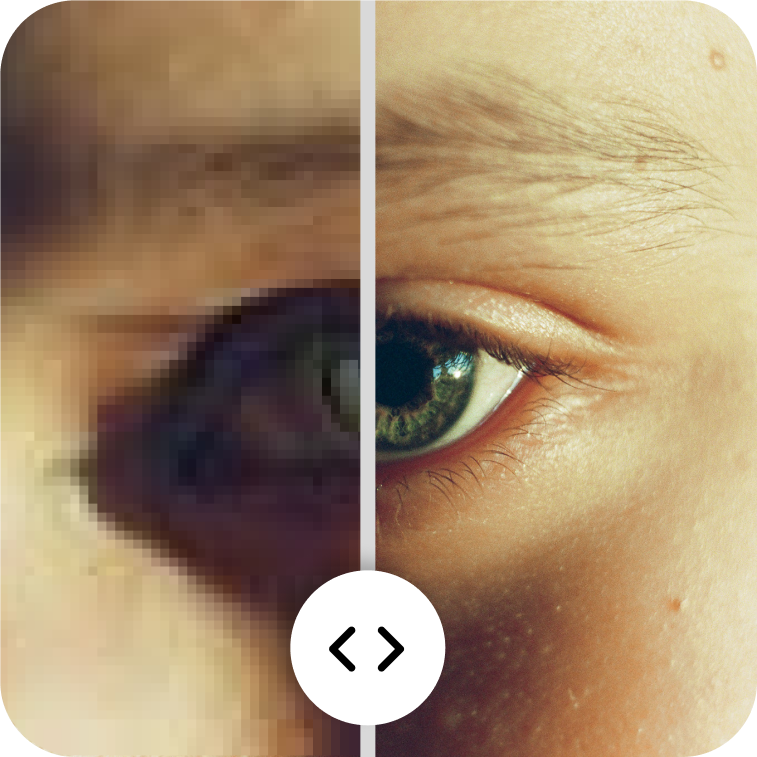
\includegraphics[width=0.2\linewidth]{Rozdziały/06.Aplikacja/Obrazy/slider.png}  
    %     \caption{Suwak prezentujący obraz przed i po przetworzeniu}
    %     \label{fig:image95}
    % \end{figure}
    \item Kolejną dużą zmianą będzie możliwość dodania do aplikacji kilku obrazów jednocześnie w celu powiększenia rozdzielczości. Ta zmiana wymaga modyfikacji w Backendzie, ponieważ obecnie aplikacja obsługuje przyjęcie i przechowanie tylko jednego obrazu na raz.
\end{itemize}

\subsection*{Usprawnienia widoku z wynikami}

\begin{itemize}
    \item Przede wszystkim chciałbym dodać możliwość wyświetlenia kilku obrazów po przetworzeniu. Obecnie widok wyświetla tylko jeden obraz, ale możliwość przedstawienia użytkownikowi wielu obrazów byłaby użyteczna i praktyczna. Możliwa implementacja jak na obrazie \ref{fig:image97}, lub integracja tej części interfejsu w pasku bocznym.
    \item Kolejną zmianą będzie lekka zmiana UI związanego z kursorem i szkłem powiększającym. Chciałbym żeby design całej aplikacji był spójny, więc dobrym pomysłem byłaby implementacja mechanizmów kursora z głównego ekranu do tego widoku. Dodatkowo myślę, że szkło powiększające powinno wyświetlać przybliżony fragment obrazu przy kursorze a nie wyłącznie na pasku bocznym, byłoby to bardziej intuicyjne dla użytkownika [Rys \ref{fig:image96}].
    % \begin{figure}[H]
    %     \centering
    %     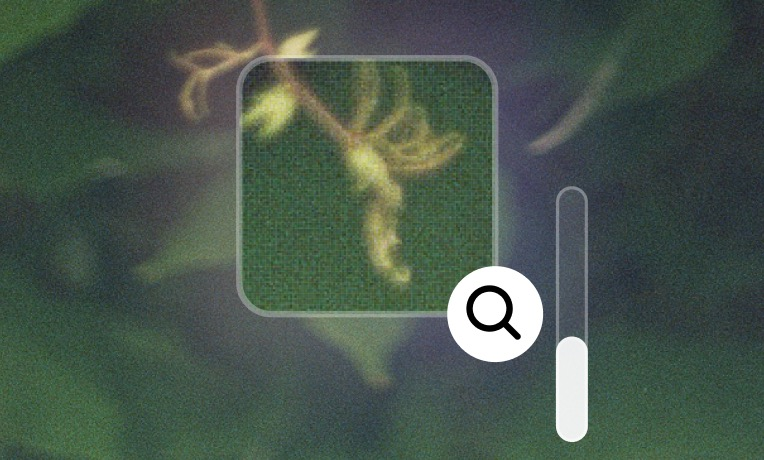
\includegraphics[width=0.2\linewidth]{Rozdziały/06.Aplikacja/Obrazy/concept-zoom.jpg}
    %     \caption{Koncepcja szkła powiększającego}
    %     \label{fig:image96}
    % \end{figure}
    \item Kolejną kwestią będzie optymalizacja wyświetlania obrazów. Obecnie obrazy są wyświetlane w pełnej rozdzielczości i w formacie oryginalnym, co jest niepotrzebne i powoduje spowolnienie działania aplikacji. W przyszłości chciałbym dodać mechanizm, który będzie wyświetlał obrazy w zależności od rozdzielczości ekranu użytkownika i w formacie webp, który jest mniej zasobożerny.
    \item Ostatnią zmianą będzie ulepszenie animacji ładowania tak żeby użytkownik wiedział, że aplikacja pracuje nad przetworzeniem obrazu. Obecnie animacja jest bardzo prosta i nie daje użytkownikowi żadnej informacji o tym co się dzieje.
\end{itemize}

\begin{figure}[ht]
    \centering
    \begin{minipage}[t]{0.3\linewidth}
        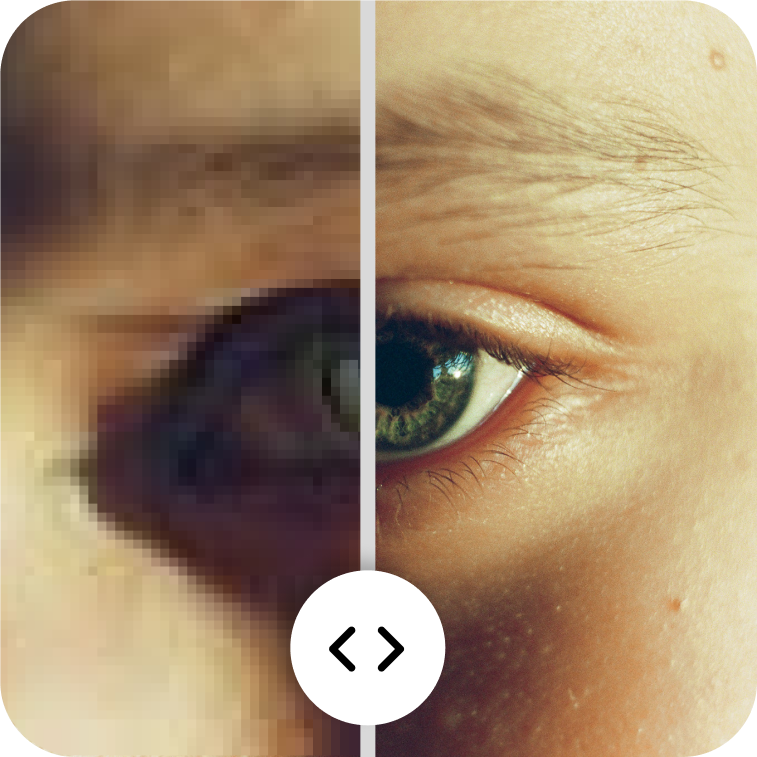
\includegraphics[width=\linewidth]{Rozdziały/06.Aplikacja/Obrazy/slider.png}
        \caption{Suwak pokazujący obraz przed i po}
        \label{fig:image95}
    \end{minipage}
    \hspace{0.5cm}
    \begin{minipage}[t]{0.5\linewidth}
        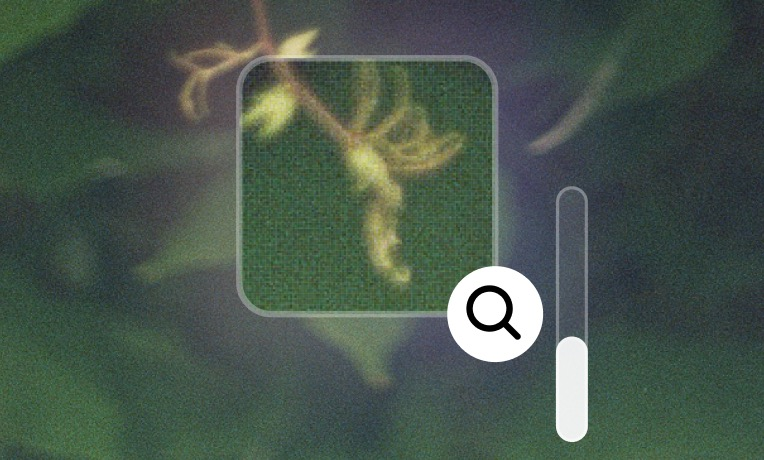
\includegraphics[width=\linewidth]{Rozdziały/06.Aplikacja/Obrazy/concept-zoom.jpg}
        \caption{Koncepcja szkła powiększającego}
        \label{fig:image96}
    \end{minipage}
\end{figure}
\begin{figure}[H]
    \centering
    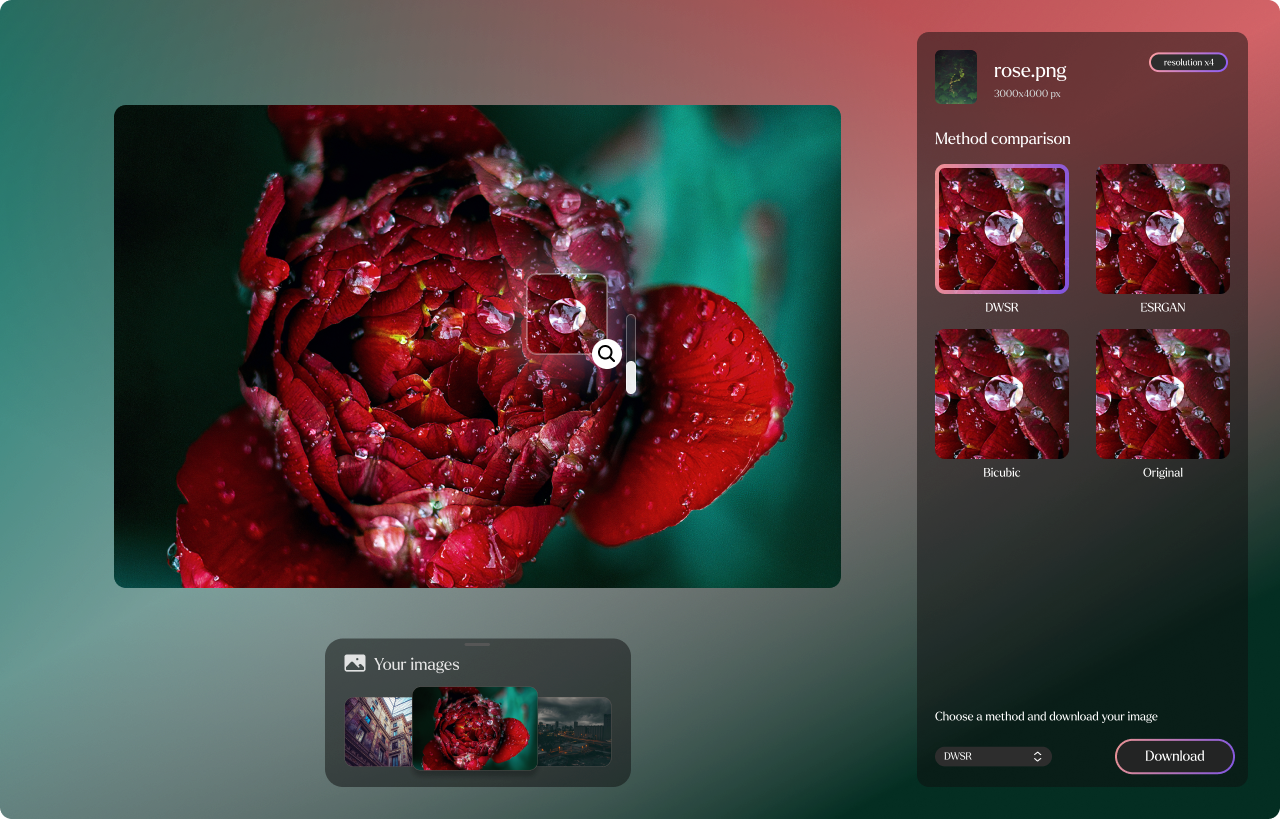
\includegraphics[width=0.9\linewidth]{Rozdziały/06.Aplikacja/Obrazy/concept-display.png}
    \caption{Koncepcja widoku prezentacji wyników z obsługą wielu obrazów jednocześnie (obraz z \cite{guo2017deep})}
    \label{fig:image97}
\end{figure}



\subsection*{Zmiany obejmujące całą aplikację}

W tym dziale przedstawię jakie zmiany obejmujące cały projekt chciałbym wprowadzić i dlaczego.

\begin{itemize}
    \item Pierwszą i najważniejszą zmianą ogólną w aplikacji będzie lepsza obsługa błędów. Póki co gdy coś jest nie tak przeglądarka wyświetla komunikat o błędzie, który jest czytelny dla mnie, ale nie dla użytkownika. W przyszłości chciałbym dodać własne komunikaty o błędach, które będą bardziej przyjazne dla użytkownika.
    \item Jedną z istotniejszych zmian w aplikacji będzie ukrycie id obrazka, gdyż w aktualnej wersji możemy przeglądać wszystkie obrazy w bazie danych na podstawie numeru ID w adresie. 
    \item Kolejną rzeczą wymagającą sporo pracy będzie dostosowanie aplikacji do urządzeń mobilnych. Obecnie aplikacja wyświetla się poprawnie tylko na komputerach, ale w przyszłości chciałbym żeby interfejs użytkownika był dostosowany również do urządzeń mobilnych.
    \item Kolejną zmianą będzie modyfikacja backendu, tak żeby serwer obsługiwał przesłanie więcej niż jednego obrazu jednocześnie. 
    \item A propos Backendu, chciałbym żeby serwer nie przechowywał wszystkich obrazów w bazie danych, tylko po zamknięciu sesji żeby obrazy były usuwane.
    \item Następną zmianą będzie dodanie dwóch widoków: dokumentacji i o mnie. Widok dokumentacji wydaje mi się konieczny w tego typu projekcie, bo chciałbym w nim odnieść się do autorów wykorzystanych rozwiązań i podziękować im za ich pracę. Widok o mnie jest opcjonalny, ale chciałbym go dodać, aby użytkownik mógł dowiedzieć się więcej o mojej pracy i miał możliwość skontaktowania się ze mną.
    \item Ostatnią kwestią gdy już uda się zaimplementować wszystkie funkcjonalności będzie udostępnienie tej aplikacji w Internecie.
\end{itemize}